\documentclass[a4paper,12pt,twoside,onecolumn,openright,final,oldfontcommands]{memoir}
\usepackage{lmodern}
\usepackage{amssymb,amsmath}
\usepackage{ifxetex,ifluatex}
\usepackage{fixltx2e} % provides \textsubscript
\ifnum 0\ifxetex 1\fi\ifluatex 1\fi=0 % if pdftex
  \usepackage[T1]{fontenc}
  \usepackage[utf8]{inputenc}
\else % if luatex or xelatex
  \ifxetex
    \usepackage{mathspec}
  \else
    \usepackage{fontspec}
  \fi
  \defaultfontfeatures{Ligatures=TeX,Scale=MatchLowercase}
\fi
% use upquote if available, for straight quotes in verbatim environments
\IfFileExists{upquote.sty}{\usepackage{upquote}}{}
% use microtype if available
\IfFileExists{microtype.sty}{%
\usepackage{microtype}
\UseMicrotypeSet[protrusion]{basicmath} % disable protrusion for tt fonts
}{}
\usepackage[unicode=true]{hyperref}
\hypersetup{
            pdftitle={From the mechanistic modeling of signaling pathways in cancer to the interpretation of models and their contributions: clinical applications and statistical evaluation},
            pdfborder={0 0 0},
            breaklinks=true}
\urlstyle{same}  % don't use monospace font for urls
\usepackage{natbib}
\bibliographystyle{plainnat}
\usepackage{longtable,booktabs}
\usepackage{graphicx,grffile}
\makeatletter
\def\maxwidth{\ifdim\Gin@nat@width>\linewidth\linewidth\else\Gin@nat@width\fi}
\def\maxheight{\ifdim\Gin@nat@height>\textheight\textheight\else\Gin@nat@height\fi}
\makeatother
% Scale images if necessary, so that they will not overflow the page
% margins by default, and it is still possible to overwrite the defaults
% using explicit options in \includegraphics[width, height, ...]{}
\setkeys{Gin}{width=\maxwidth,height=\maxheight,keepaspectratio}
\IfFileExists{parskip.sty}{%
\usepackage{parskip}
}{% else
\setlength{\parindent}{0pt}
\setlength{\parskip}{6pt plus 2pt minus 1pt}
}
\setlength{\emergencystretch}{3em}  % prevent overfull lines
\providecommand{\tightlist}{%
  \setlength{\itemsep}{0pt}\setlength{\parskip}{0pt}}
\setcounter{secnumdepth}{5}
% Redefines (sub)paragraphs to behave more like sections
\ifx\paragraph\undefined\else
\let\oldparagraph\paragraph
\renewcommand{\paragraph}[1]{\oldparagraph{#1}\mbox{}}
\fi
\ifx\subparagraph\undefined\else
\let\oldsubparagraph\subparagraph
\renewcommand{\subparagraph}[1]{\oldsubparagraph{#1}\mbox{}}
\fi
%%%%%%%%%%%%%%%%%%%%%%%%%%%%%%%%%%%%%%%%%%%%%%%%%%%%%%%%%%%%%
%Start preamble
%%%%%%%%%%%%%%%%%%%%%%%%%%%%%%%%%%%%%%%%%%%%%%%%%%%%%%%%%%%%%

\usepackage{booktabs}
\usepackage{amsthm}
\usepackage{./cover/psl-cover} % specifies the path to the cover page template

%\makeatletter
%\def\thm@space@setup{%
%  \thm@preskip=8pt plus 2pt minus 4pt
%  \thm@postskip=\thm@preskip
%}
%\makeatother


%%%%%%%%%%%%%%%%%%%%%%%%%%%%%%%%%%%%%%%%%%%%%%%%%%%%%%%%%%%%%
% Add a lettrine to the very first character of the content %
%%%%%%%%%%%%%%%%%%%%%%%%%%%%%%%%%%%%%%%%%%%%%%%%%%%%%%%%%%%%%

\usepackage{lettrine} % supports various dropped capitals styles

\newcommand{\initial}[1]{
	\lettrine[lines=3,lhang=0.33,nindent=0em]{
		\color{gray}
     		{\textsc{#1}}}{}}
     		
%%%%%%%%%%%%%%%%%%%%%%%%
% Insert an empty page %
%%%%%%%%%%%%%%%%%%%%%%%%

\usepackage{afterpage} % executes command after the next page break

\newcommand\blankpage{%
    \null
    \thispagestyle{empty}%
    % \addtocounter{page}{-1}% % uncomment to increase page counter
    \newpage
    }

\newcommand{\clearemptydoublepage}{\newpage{\thispagestyle{empty}\cleardoublepage}}

%%%%%%%%%%%%%%%%%%
% Epigraph style %
%%%%%%%%%%%%%%%%%%

\usepackage{epigraph} % provides commands to assist in the typesetting of a single epigraph

\setlength\epigraphwidth{1\textwidth}
\setlength\epigraphrule{0pt} % no line between
\setlength\beforeepigraphskip{1\baselineskip} % space before and after epigraph
\setlength\afterepigraphskip{2\baselineskip}
\renewcommand*{\textflush}{flushright}
\renewcommand*{\epigraphsize}{\normalsize\itshape}

%%%%%%%%%%%%%%%%%%%%%%%%
% Formatting
%%%%%%%%%%%%%%%%%%%%

\usepackage{calc} % simple arithmetics in latex commands
\usepackage{soul} % hyphenation for letterspacing, underlining, etc.

\makeatletter
\newlength\dlf@normtxtw
\setlength\dlf@normtxtw{\textwidth}
\newsavebox{\feline@chapter}
\newcommand\feline@chapter@marker[1][4cm]{%
	\sbox\feline@chapter{%
		\resizebox{!}{#1}{\fboxsep=1pt%
			\colorbox{gray}{\color{white}\thechapter}%
		}}%
		\rotatebox{90}{%
			\resizebox{%
				\heightof{\usebox{\feline@chapter}}+\depthof{\usebox{\feline@chapter}}}%
			{!}{\scshape\so\@chapapp}}\quad%
		\raisebox{\depthof{\usebox{\feline@chapter}}}{\usebox{\feline@chapter}}%
}

\newcommand\feline@chm[1][4cm]{%
	\sbox\feline@chapter{\feline@chapter@marker[#1]}%
	\makebox[0pt][c]{% aka \rlap
		\makebox[1cm][r]{\usebox\feline@chapter}%
	}}

\makechapterstyle{daleifmodif}{
\renewcommand\chapnamefont{\normalfont\Large\scshape\raggedleft\so}
\renewcommand\chaptitlefont{\normalfont\Large\bfseries\scshape}
\renewcommand\chapternamenum{} \renewcommand\printchaptername{}
\renewcommand\printchapternum{\null\hfill\feline@chm[2.5cm]\par}
\renewcommand\afterchapternum{\par\vskip\midchapskip}
\renewcommand\printchaptertitle[1]{\color{gray}\chaptitlefont\raggedleft
  \renewcommand\chaptername{Chapter}
  ##1\par}
}

\makeatother
\chapterstyle{daleifmodif}

% The pages should be numbered consecutively at the bottom centre of the page
\makepagestyle{myvf}
\makeoddfoot{myvf}{}{\thepage}{}
\makeevenfoot{myvf}{}{\thepage}{}
\makeheadrule{myvf}{\textwidth}{\normalrulethickness}
\makeevenhead{myvf}{\small\textsc{\leftmark}}{}{}
\makeoddhead{myvf}{}{}{\small\textsc{\rightmark}}
\pagestyle{myvf}


%%%%%%%%%%%%%%%%%%%%%%%%%%%%%%%%%%%%%%%%%%%%%%%%%%%%%%%%%%%%%
% Define cover page settings
%%%%%%%%%%%%%%%%%%%%%%%%%%%%%%%%%%%%%%%%%%%%%%%%%%%%%%%%%%%%%

\title{My title}

\author{Jonas BEAL}

\institute{l'Institut Curie}
\doctoralschool{Complexite du Vivant}{515}

\institute{l'Institut Curie}
\doctoralschool{Complexité du Vivant}{515}
\specialty{Génomique}
\date{23 septembre 2020}

%% cotutelle
% \entitle{Thesis Subject in English}
% \otherinstitute{CEA Saclay}
% \logootherinstitute{logo-institute}

\jurymember{1}{Test NOM}{Titre, Établissement}{Rapporteur}
\jurymember{2}{Test NOM}{Titre, Établissement}{Rapporteur}
\jurymember{3}{Test NOM}{Titre, Établissement}{Examinateur}
\jurymember{4}{Test NOM}{Titre, Établissement}{Examinateur}
\jurymember{5}{Emmanuel BARILLOT}{Institut Curie, INSERM, Mines ParisTech, PSL}{Directeur de thèse}
\jurymember{6}{Aurélien LATOUCHE}{Institut Curie, Cnam}{Directeur de thèse}
\jurymember{7}{Laurence CALZONE}{Institut Curie, INSERM, Mines ParisTech, PSL}{Co-encadrante de thèse}
% \jurymember{9}{Prénom NOM}{Titre, établissement}{Invité}
% \jurymember{10}{Prénom NOM}{Titre, établissement}{Invité}

\frabstract{
  Au delà de ses mécanismes génétiques, le cancer peut-être compris comme une maladie de réseaux qui résulte souvent de l’interaction entre différentes perturbations dans un réseau de régulation cellulaire.  La dynamique de ces réseaux et des voies de signalisation associées est complexe et requiert des approches intégrées. Une d’entre elles est la conception de modèles dits mécanistiques qui traduisent mathématiquement la connaissance biologique des réseaux afin de pouvoir simuler le fonctionnement moléculaire des cancers informatiquement. Ces modèles ne traduisent cependant que les mécanismes généraux à l’oeuvre dans certains cancers en particulier.

Cette thèse propose en premier lieu de définir des modèles mécanistiques personnalisés de cancer. Un modèle générique est  d’abord défini dans un formalisme logique (ou Booléen), avant d’utiliser les données omiques (mutations, ARN, protéines) de patients ou de lignées cellulaires afin de rendre le modèle spécifique à chacun. Ces modèles personnalisés peuvent ensuite être confrontés aux données cliniques de patients pour vérifier leur validité. Le cas de la réponse clinique aux traitements est exploré en particulier dans cette thèse. La représentation explicite des mécanismes moléculaires par ces modèles permet en effet de simuler l’effet de différents traitements suivant leur mode d’action et de vérifier si la sensibilité d’un patient à un traitement est bien prédite par le modèle personnalisé correspondant. Un exemple concernant la réponse aux inhibiteurs de BRAF dans les mélanomes et cancers colorectaux est ainsi proposé.

La confrontation des modèles mécanistiques de cancer, ceux présentés dans cette thèse et d’autres, aux données cliniques incite par ailleurs à évaluer rigoureusement leurs éventuels bénéfices dans la cadre d’une utilisation médicale. La quantification et l’interprétation de la valeur de certains modèles à visée pronostique est brièvement présentée avant de se focaliser sur le cas particulier des modèles capables de sélectionner le meilleur traitement pour chaque patient en fonction des ses caractéristiques moléculaires. Un cadre théorique est proposé pour étendre les méthodes d’inférence causale à l’évaluation de tels algorithmes de médecine de précision. Une illustration est fournie à l’aide de données simulées et de xénogreffes dérivées de  patients

L’ensemble des méthodes et applications décrites tracent donc un chemin, de la conception de modèles mécanistiques de cancer à leur évaluation grâce à des modèles statistiques émulant des essais cliniques.

}

\enabstract{
  Beyond its genetic mechanisms, cancer can be understood as a network disease that often results from the interaction between different perturbations in a cellular regulatory network.  The dynamics of these networks and associated signaling pathways are complex and require integrated approaches. One approach is to design mechanistic models that translate the biological knowledge of networks in mathematical terms to simulate the molecular features of cancers in a computer-readable form. However, these models only reflect the general mechanisms at work in cancers.

This thesis proposes to define personalized mechanistic models of cancer. A generic model is first defined in a logical (or Boolean) formalism, before using omics data (mutations, RNA, proteins) from patients or cell lines in order to make the model specific to each one profile. These personalized models can then be compared with the clinical data of patients in order to validate them. The response to treatment is investigated in particular in this thesis. The explicit representation of the molecular mechanisms by these models allows to simulate the effect of different treatments according to their targets and to verify if the sensitivity of a patient to a drug is well predicted by the corresponding personalized model. An example concerning the response to BRAF inhibitors in melanomas and colorectal cancers is thus presented.

The comparison of mechanistic models of cancer, those presented in this thesis and others, with clinical data also encourages a rigorous evaluation of their possible benefits in the context of medical use. The quantification and interpretation of the value of certain prognostic models is briefly presented before focusing on the particular case of models able to recommend the best treatment for each patient according to his molecular profile. A theoretical framework is defined to extend causal inference methods to the evaluation of such precision medicine algorithms. An illustration is provided using simulated data and patient derived xenografts.

All the methods and applications put forward a possible path from the design of mechanistic models of cancer to their evaluation using statistical models emulating clinical trials.

}

\frkeywords{ Modélisation, Cancer, Modèle mécanistique, Biostatistiques, Inférence causale, Médecine de précision.}
\enkeywords{ Modeling, Cancer, Mechanistic model, Biostatistics, Causal inference, Precision medicine.}
  
\pagenumbering{roman}
\usepackage{booktabs}
\usepackage{longtable}
\usepackage{array}
\usepackage{multirow}
\usepackage{wrapfig}
\usepackage{float}
\usepackage{colortbl}
\usepackage{pdflscape}
\usepackage{tabu}
\usepackage{threeparttable}
\usepackage{threeparttablex}
\usepackage[normalem]{ulem}
\usepackage{makecell}
\usepackage{xcolor}

\title{From the mechanistic modeling of signaling pathways in cancer to the
interpretation of models and their contributions: clinical applications
and statistical evaluation}
\date{23/09/2020}

\begin{document}
\maketitle

\chapter*{Abstract}

\initial{B}eyond its genetic mechanisms, cancer can be understood as a
network disease that often results from the interaction between
different perturbations in a cellular regulatory network. The dynamics
of these networks and associated signaling pathways are complex and
require integrated approaches. One approach is to design mechanistic
models that translate the biological knowledge of networks in
mathematical terms to simulate the molecular features of cancers in a
computer-readable form. However, these models only reflect the general
mechanisms at work in cancers.

This thesis proposes to define personalized mechanistic models of
cancer. A generic model is first defined in a logical (or Boolean)
formalism, before using omics data (mutations, RNA, proteins) from
patients or cell lines in order to make the model specific to each one
profile. These personalized models can then be compared with the
clinical data of patients in order to validate them. The response to
treatment is investigated in particular in this thesis. The explicit
representation of the molecular mechanisms by these models allows to
simulate the effect of different treatments according to their targets
and to verify if the sensitivity of a patient to a drug is well
predicted by the corresponding personalized model. An example concerning
the response to BRAF inhibitors in melanomas and colorectal cancers is
thus presented.

The comparison of mechanistic models of cancer, those presented in this
thesis and others, with clinical data also encourages a rigorous
evaluation of their possible benefits in the context of medical use. The
quantification and interpretation of the value of certain prognostic
models is briefly presented before focusing on the particular case of
models able to recommend the best treatment for each patient according
to his molecular profile. A theoretical framework is defined to extend
causal inference methods to the evaluation of such precision medicine
algorithms. An illustration is provided using simulated data and patient
derived xenografts.

All the methods and applications put forward a possible path from the
design of mechanistic models of cancer to their evaluation using
statistical models emulating clinical trials.

\vspace{\baselineskip}

\textbf{Key-words}: Modeling, Cancer, Mechanistic model, Biostatistics,
Causal inference, Precision medicine

\chapter*{Résumé}

\initial{A}u delà de ses mécanismes génétiques, le cancer peut-être
compris comme une maladie de réseaux qui résulte souvent de
l'interaction entre différentes perturbations dans un réseau de
régulation cellulaire. La dynamique de ces réseaux et des voies de
signalisation associées est complexe et requiert des approches
intégrées. Une d'entre elles est la conception de modèles dits
mécanistiques qui traduisent mathématiquement la connaissance biologique
des réseaux afin de pouvoir simuler le fonctionnement moléculaire des
cancers informatiquement. Ces modèles ne traduisent cependant que les
mécanismes généraux à l'oeuvre dans certains cancers en particulier.

Cette thèse propose en premier lieu de définir des modèles mécanistiques
personnalisés de cancer. Un modèle générique est d'abord défini dans un
formalisme logique (ou Booléen), avant d'utiliser les données omiques
(mutations, ARN, protéines) de patients ou de lignées cellulaires afin
de rendre le modèle spécifique à chacun. Ces modèles personnalisés
peuvent ensuite être confrontés aux données cliniques de patients pour
vérifier leur validité. Le cas de la réponse clinique aux traitements
est exploré en particulier dans cette thèse. La représentation explicite
des mécanismes moléculaires par ces modèles permet en effet de simuler
l'effet de différents traitements suivant leur mode d'action et de
vérifier si la sensibilité d'un patient à un traitement est bien prédite
par le modèle personnalisé correspondant. Un exemple concernant la
réponse aux inhibiteurs de BRAF dans les mélanomes et cancers
colorectaux est ainsi proposé.

La confrontation des modèles mécanistiques de cancer, ceux présentés
dans cette thèse et d'autres, aux données cliniques incite par ailleurs
à évaluer rigoureusement leurs éventuels bénéfices dans la cadre d'une
utilisation médicale. La quantification et l'interprétation de la valeur
de certains modèles à visée pronostique est brièvement présentée avant
de se focaliser sur le cas particulier des modèles capables de
sélectionner le meilleur traitement pour chaque patient en fonction des
ses caractéristiques moléculaires. Un cadre théorique est proposé pour
étendre les méthodes d'inférence causale à l'évaluation de tels
algorithmes de médecine de précision. Une illustration est fournie à
l'aide de données simulées et de xénogreffes dérivées de patients.

L'ensemble des méthodes et applications décrites tracent donc un chemin,
de la conception de modèles mécanistiques de cancer à leur évaluation
grâce à des modèles statistiques émulant des essais cliniques.

\vspace{\baselineskip}

\textbf{Mots-clés}: Modélisation, Cancer, Modèle mécanistique,
Biostatistiques, Inférence causale, Médecine de précision

\afterpage{\blankpage}

\chapter*{Acknowledgements}

\initial{M}any persons to thanks. Lorem ipsum dolor sit amet,
consectetur adipiscing elit, sed do eiusmod tempor incididunt ut labore
et dolore magna aliqua. Ut enim ad minim veniam, quis nostrud
exercitation ullamco laboris nisi ut aliquip ex ea commodo consequat.

Duis aute irure dolor in reprehenderit in voluptate velit esse cillum
dolore eu fugiat nulla pariatur. Excepteur sint occaecat cupidatat non
proident, sunt in culpa qui officia deserunt mollit anim id est laborum

\clearemptydoublepage

\chapter*{Preface}

\initial{T}he present thesis is structured in three parts, each
subdivided into three chapters. Since the whole thesis is about cancer
modeling, the first part aims at defining the type of model to be
referred to, and in particular models that will be called mechanistic,
as well as the object of the modeling, i.e.~the molecular networks
involved in cancer. So the first part answers the question: \textbf{what
is a cancer model and what is its purpose?}

The second part will be devoted to the methods developed during this
thesis to transform qualitative models of molecular networks, known as
logic models, into personalized models that can be interpreted
clinically. In short, \textbf{how can a mathematical representation of
biological knowledge be transformed into a tool that contributes to the
understanding of the clinical manifestations of cancer?}

Finally, the third and last part will look at how the clinical relevance
of all the above-mentioned models can be rigorously evaluated, both in
their ability to predict the evolution of the disease and in their
ability to recommend the most appropriate treatments for each patient.
\textbf{How to quantify and interpret the value of the clinical
information delivered by these models?}

Moreover, this thesis also exists in an online version that allows to
take advantage of the interactivity of some graphs and applications:
\url{https://jonasbeal.github.io/thesis/}.

\clearemptydoublepage

\renewcommand{\contentsname}{Table of contents}

\maxtocdepth{subsection}

\tableofcontents*
\addtocontents{toc}{\par\nobreak \mbox{}\hfill{\bf Page}\par\nobreak}
\newpage

\listoftables
\addtocontents{lot}{\par\nobreak\textbf{{\scshape Table} \hfill Page}\par\nobreak}
\newpage

\listoffigures
\addtocontents{lof}{\par\nobreak\textbf{{\scshape Figure} \hfill Page}\par\nobreak}
\newpage

\blankpage

\pagenumbering{arabic}

\part{Cells and their
models}\label{part-cells-and-their-models}

\chapter{Scientific modeling: abstract the
complexity}\label{scientific-modeling-abstract-the-complexity}

\epigraph{"Ce qui est simple est toujours faux. Ce qui ne l'est pas est inutilisable."}{Paul Valéry (Mauvaises pensées et autres, 1942)}

\initial{T}he notion of modeling is embedded in science, to the point
that it has sometimes been used to define the very nature of scientific
research. What is called a model can, however, correspond to very
different realities which need to be defined before addressing the
object of this thesis which will consist, if one wants to be
mischievous, in analyzing models with other models. This semantic
elucidation is all the more necessary as this thesis is
interdisciplinary, suspended between systems biology and biostatistics.
In order to convince the reader of the need for such a preamble, he is
invited to ask a statistician and a biologist how they would define what
a model is.

\begin{figure}

{\centering \includegraphics[width=0.9\linewidth]{fig/orrery} 

}

\caption[A scientist and his model]{\textbf{A scientist and his model.} Joseph Wright
of Derby, \emph{A Philosopher Giving a Lecture at the Orrery (in which a
lamp is put in place of the sun)}, c. 1763-65, oil on canvas, Derby
Museums and Art Gallery}\label{fig:orrery}
\end{figure}






\section{What is a model?}\label{what-is-a-model}

\subsection{In your own words}\label{in-your-own-words}

A model is first of all an ambiguous object and a polysemous word. It
therefore seems necessary to start with a semantic study. Among the many
meanings and synonymous proposed by the dictionary (Figure
\ref{fig:visual-thesaurus}), while some definitions are more related to
art, several find echoes in scientific practice. It is sometimes a
question of the physical representation of an object, often on a reduced
scale as in Figure \ref{fig:orrery}, and sometimes of a theoretical
description intended to facilitate the understanding of the way in which
a system works \citep{dictionnarymodel}. It is even sometimes an ideal
to be reached and therefore an ambitious prospect for an introduction.

\begin{figure}

{\centering 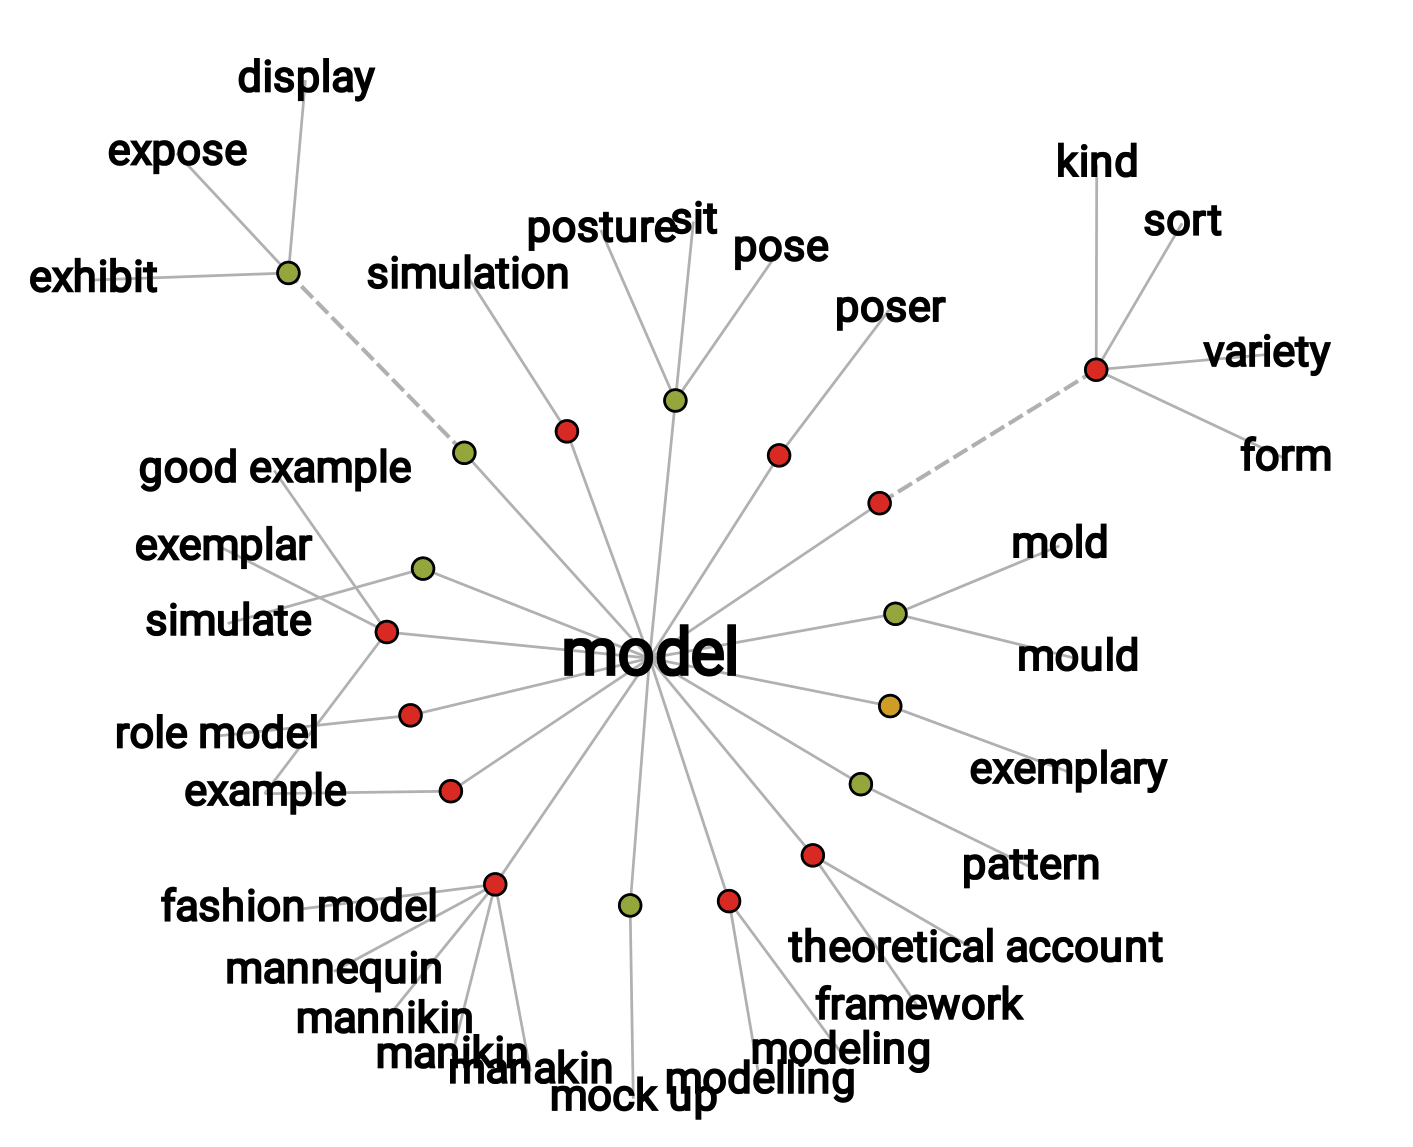
\includegraphics[width=0.9\linewidth]{fig/visualThesaurus} 

}

\caption[Network visualization of *model* thesaurus entries]{\textbf{Network visualization of
\emph{model} thesaurus entries.} Generated with the
\href{https://www.visualthesaurus.com}{`Visual Thesaurus'} ressource}\label{fig:visual-thesaurus}
\end{figure}





The narrower perspective of the scientist does not reduce the
completeness of the dictionary's description to an unambiguous object
\citep{bailer2002scientists}. In an attempt to approach these
multi-faceted objects that are the models, Daniela Bailer-Jones
interviewed different scientists and asked them the same question: what
is a model? Across the different profiles and fields of study, the
answers vary but some patterns begin to emerge (Figure
\ref{fig:interviews}). A model must capture the essence of the
phenomenon being studied. Because it eludes, voluntarily or not, many
details or complexity, it is by nature a simplification of the
phenomenon. These limitations may restrict its validity to certain cases
or suspend it to the fulfilment of some hypotheses. They are not
necessarily predictive, but they must be able to generate new
hypotheses, be tested and possibly questioned. Finally, and
fundamentally, they \textbf{must provide insights about the object of
study and contribute to its understanding}.

\begin{figure}

{\centering 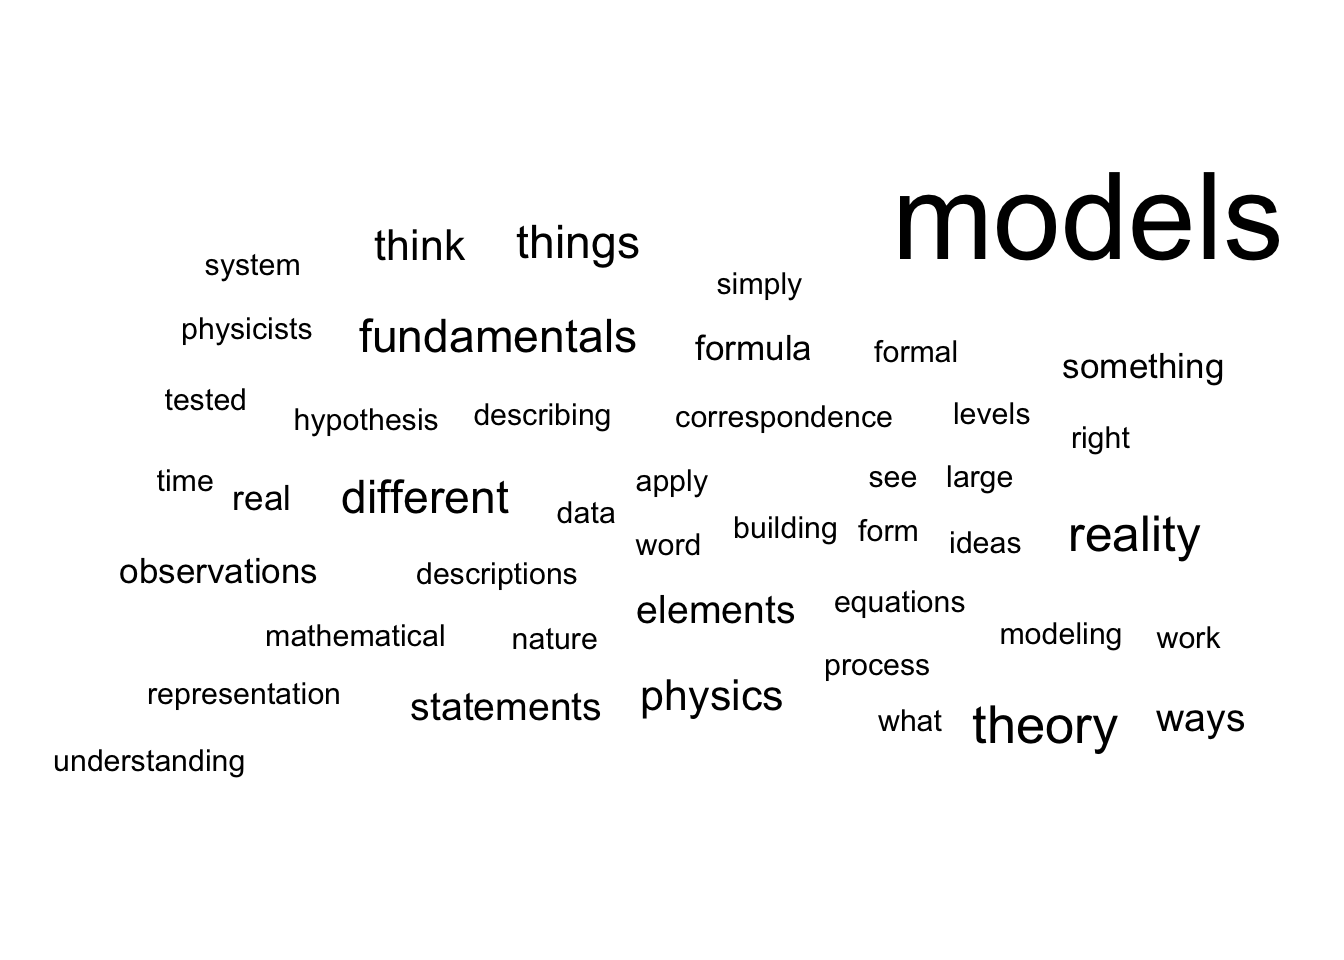
\includegraphics[width=0.9\linewidth]{01-Models_files/figure-latex/interviews-1} 

}

\caption[Scientists talk about their models: words cloud.]{\textbf{Scientists talk about their models:
words cloud.} Cloud of words summarizing the lexical fields used by
scientists to talk about their models in dedicated interviews reported
by \citet{bailer2002scientists}.}\label{fig:interviews}
\end{figure}






These definitions circumscribe the \emph{model} object, its use and its
objectives, but they do not in any way describe its nature. And for good
reason, because even if we agree on the described contours, the
biodiversity of the models remains overwhelming for taxonomists:

\begin{quote}
\emph{Probing models, phenomenological models, computational models,
developmental models, explanatory models, impoverished models, testing
models, idealized models, theoretical models, scale models, heuristic
models, caricature models, exploratory models, didactic models, fantasy
models, minimal models, toy models, imaginary models, mathematical
models, mechanistic models, substitute models, iconic models, formal
models, analogue models, and instrumental models are but some of the
notions that are used to categorize models.}\\
\citep{frigg2020models}
\end{quote}

\subsection{Physical world and world of
ideas}\label{physical-world-and-world-of-ideas}

Without claiming to be exhaustive, we can make a \textbf{first simple
dichotomy between physical/material and formal/intellectual models}
\citep{rosenblueth1945role}. The former consist in replacing the object
of study by another object, just as physical but nevertheless simpler or
better known. These may be models involving a change of scale such as
the simple miniature replica placed in a wind tunnel, or the metal
double helix model used by Watson and Crick to visualize DNA. In all
these cases the model allows to visualize the object of study (Figure
\ref{fig:planets} A and B), to manipulate it and play with it to better
understand or explain a phenomenon, just like the scientist with his
orrery (Figure \ref{fig:orrery}). In the case of biology, there are
mainly model organisms such as drosophila, zebrafish or mice, for
example. We then benefit from the relative simplicity of their genomes,
a shorter time scale or ethical differences, usually to elucidate
mechanisms of interest in humans. Correspondence between the target
system and its model can sometimes be more conceptual, such as that ones
relying on mechanical--electrical analogies: a mechanical system (e.g.~a
spring-mass system) can sometimes be represented by an electric network
(e.g.~a RLC circuit with a resistor, a capacitor and an inductor).

\begin{figure}

{\centering 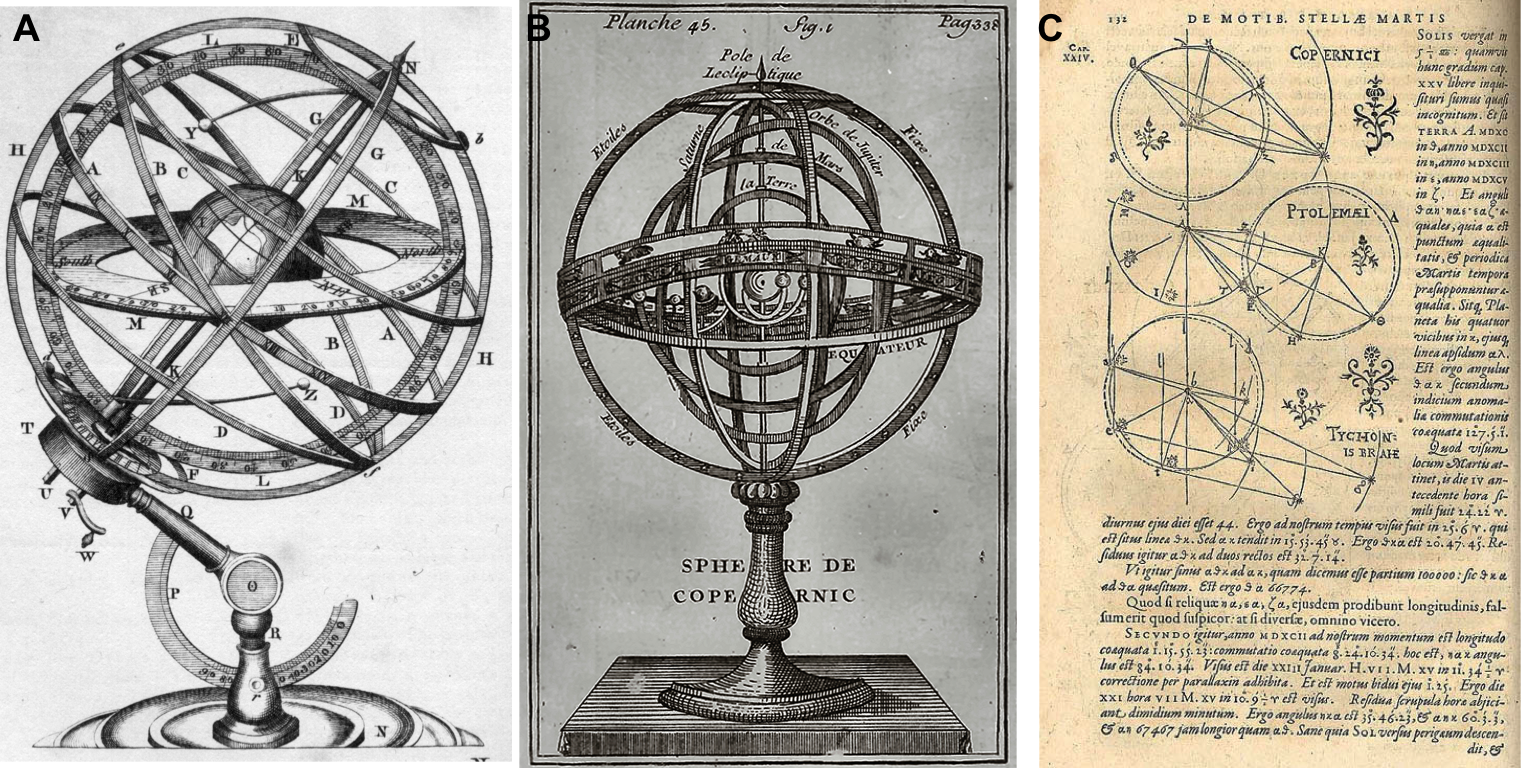
\includegraphics[width=0.9\linewidth]{01-Models_files/figure-latex/planets-1} 

}

\caption[Orrery, planets and models]{\textbf{Orrery, planets and models}. Physical
models of planetary motion, either geocentric (Armillary sphere from
\emph{Plate LXXVII} in
\href{https://commons.wikimedia.org/wiki/File:EB1711_Armillary_Sphere.png}{\emph{Encyclopedia
Britannica}}, 1771) or heliocentric in panel B (Bion, 1751,
\href{https://gallica.bnf.fr/ark:/12148/btv1b2600252q/f8.item.r=Bion}{catalogue
Bnf}) and some geometric representations by Johannes Kepler in panel C
(in
\href{https://commons.wikimedia.org/wiki/File:Kepler_astronomia_nova.jpg}{\emph{Astronomia
Nova}}, 1609)}\label{fig:planets}
\end{figure}












The model is then no longer simply a mimetic replica but is based on an
intellectual equivalence: we are gradually moving into the realm of
formal models \citep{rosenblueth1945role}. These are of a more symbolic
nature and they \textbf{represent the original system with a set of
logical or mathematical terms}, describing the main driving forces or
similar structural properties as geometrical models of planetary motions
summarized by Kepler in Figure \ref{fig:planets}C. Historically these
models have often been expressed by sets of mathematical equations or
relationships. Increasingly, these have been implemented by computer.
Despite their sometimes less analytical and more numerical nature, many
so-called computational models could also belong to this category of
formal models. There are then many formalisms, discrete or continuous,
deterministic or stochastic, based on differential equations or Boolean
algebra \citep{fowler1997mathematical}. Despite their more abstract
nature, they offer similar scientific services: it is possible to play
with their parameters, specifications or boundary conditions in order to
better understand the phenomenon. One can also imagine these formal
models from a different perspective, which starts from the data in a
bottom-up approach instead of starting from the phenomenon in a top-down
analysis. These models will then often be called statistical models or
models of data \citep{frigg2020models}. This distinction will be further
clarified in section \ref{stat-mech}.

To summarize and continue a little longer with the astronomical
metaphor, the study of a particularly complex system (the solar system)
can be broken down into a variety of different models. Physical and
mechanical models such as armillary spheres (\ref{fig:planets}A and B)
make it possible to touch the object of study. In addition, we can
observe the evolution of models which, when confronted with data, have
progressed from a geocentric to a heliocentric representation to get
closer to the current state of knowledge. Sometimes, models with more
formal representations are used to give substance to ideas and
hypotheses (\ref{fig:planets}C). One of the most conceptual forms is
then the mathematical language and one can thus consider that the
previously mentioned astronomical models find their culmination in
Kepler's equations about orbits, areas and periods that describe the
elliptical motion of the planets. We refer to them today as Kepler's
laws. The model has become a law and therefore a paragon of mathematical
modeling \citep{wan2018mathematical}.

\subsection{Preview about cancer
models}\label{preview-about-cancer-models}

As we get closer to the subject of our study, and in order to illustrate
these definitions more concretely, we can take an interest in the
meaning of the word \emph{model} in the context of cancer research. For
this, we restrict our corpus to scientific articles found when searching
for ``cancer model'' in the PubMed article database. Among these, we
look at the occurrences of the word \emph{model} and the sentences in
which it is included. This cancer-related context of model is
represented as a tree in Figure \ref{fig:pubmed-tree}. Some of the
distinctions already mentioned can be found here. The \emph{mouse} and
\emph{xenograft} models, which will be discussed later in this thesis,
represent some of the most common physical models in cancer studies.
These are animal models in which the occurrence and mechanisms of
cancer, usually induced by the biologist, are studied. On the other
hand, \emph{prediction}, \emph{prognostic} or \emph{risk score} models
refer to formal models and borrow from statistical language.

\begin{figure}

{\centering 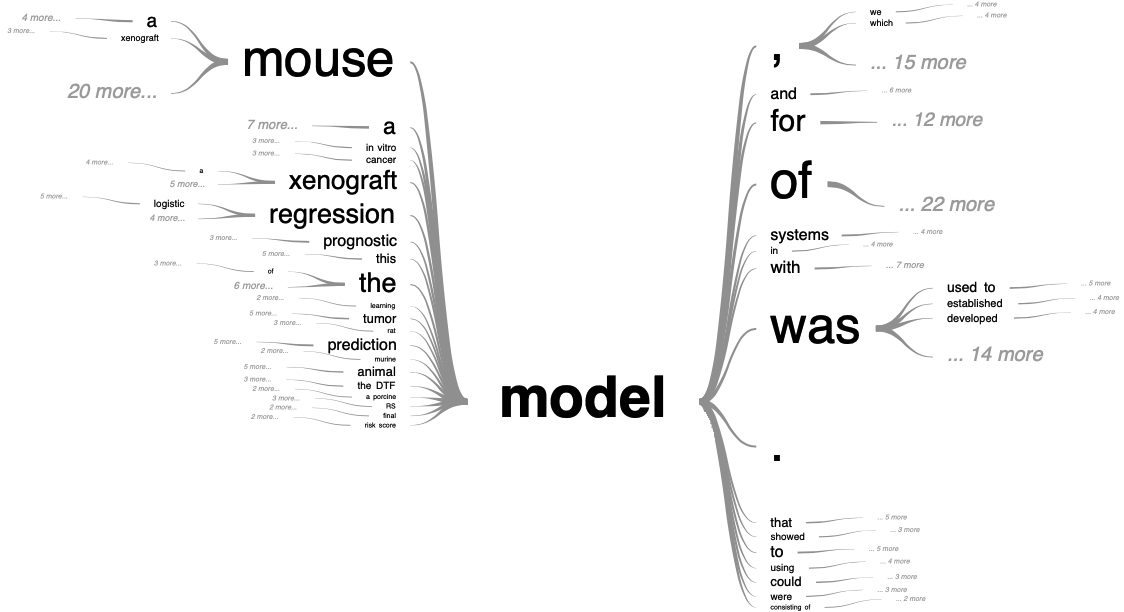
\includegraphics[width=0.9\linewidth]{fig/pubmed-tree} 

}

\caption[Tree visualization of *model* semantic context in cancer-related literature]{\textbf{Tree visualization of \emph{model}
semantic context in cancer-related literature} Generated with the
\href{https://esperr.github.io/pub-trees/}{`PubTrees'} tool by Ed Sperr,
and based on most relevant PubMed entries for ``cancer model'' search.}\label{fig:pubmed-tree}
\end{figure}






Another way to classify cancer models may be to group them into the
following categories: \emph{in vivo}, \emph{in vitro} and \emph{in
silico}. The first two clearly belong to the physical models but one
uses whole living organisms (e.g.~a human tumour implanted in an
immunodeficient mouse) and the other separates the living from its
organism in order to place it in a controlled environment (e.g.~tumour
cells in growth medium in a Petri dish). \textbf{In the thesis, data
from both \emph{in vivo} and \emph{in vitro} models will be used.
However, unless otherwise stated, a model will always refer to a
representation \emph{in silico}.} This third category, however, contains
a very wide variety of models \citep{deisboeck2009silico}, to which we
will come back in chapter \ref{mechanistic-cancer}. A final ambiguity
about the nature of the formal models used in this thesis needs to be
clarified beforehand.

\section{Statistics or mechanistic}\label{stat-mech}

A rather frequent metaphor is to compare formal models to black boxes
that take in input \(X\) predictors, or independent variables, and
output response variable(s) \(Y\), also named dependent variables. The
models then split into two categories (Figure \ref{fig:boxes}) depending
on the answer to the question: are you modeling the inside of the box or
not?

\subsection{The inside of the box}\label{the-inside-of-the-box}

The purpose of this section is to present in a schematic, and therefore
somewhat caricatural, manner the two competing formal modeling
approaches that will be used in this thesis and that we will call
mechanistic modeling and statistical modeling. Assuming the unambiguous
nature of the predictors and outputs we can imagine that the natural
process consists in defining the result Y from the inputs X according to
a function of a completely unknown form (Figure \ref{fig:boxes}A).

\begin{figure}

{\centering 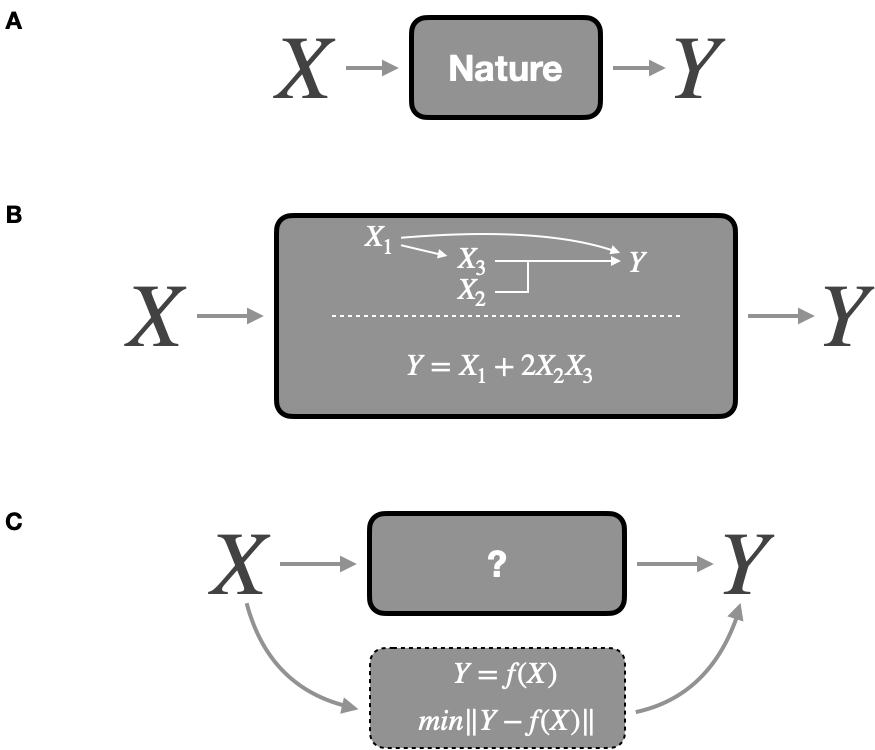
\includegraphics[width=0.6\linewidth]{fig/boxes} 

}

\caption[Different modeling strategies.]{\textbf{Different modeling strategies.} (A) Data
generation from predictors \(X\) to response \(Y\) in the natural
phenomenon. (B) Mechanistic modeling defining mechanisms of data
generation inside the box. (C) Statistical modeling finding the function
\(f\) that gives the best predictions. Aadapted from
\citet{breiman2001statistical}.}\label{fig:boxes}
\end{figure}








The first modeling approach, that we will call \textbf{mechanistic},
consists in \textbf{building the box by imitating what we think is the
process of data generation} (Figure \ref{fig:boxes}B). This integration
of a priori knowledge can take different forms. In this thesis it will
often come back to presupposing certain relations between entities
according to what is known about their behaviour. \(X_1\) which acts on
\(X_3\) may correspond to the action of one biological entity on
another, supposedly unidirectional; just as the joint action of \(X_2\)
and \(X_3\) may reflect a known synergy in the expression of genes or
the action of proteins. Mathematically this is expressed here with a
perfectly deterministic model defined a priori. All in all, in a purely
mechanistic approach, the nature of the relations between entities
should be linked to biological processes and the parameters in the model
all have biological definitions in such a way that it could even be
considered to measure them directly. For example, the coefficient \(2\)
multiplying \(X_2X_3\) can correspond to a stoichiometric coefficient or
a reaction constant which have a theoretical justification or are
accessible by experimentation. In some fields of literature these models
are sometimes called mathematical models because they propose a
mathematical translation of a phenomenon, which does not start from the
data in a bottom-up approach but rather from a top-down theoretical
framework. In this thesis we will adhere to the \emph{mechanistic model}
name, which is more transparent and less ambiguous compared to other
approaches also based on mathematics, without necessarily the other
characteristics described above.

The second approach, often called \textbf{statistical modeling}, or
sometimes machine learning depending on the precise context and
objective, does not necessarily seek to reproduce the natural process of
data generation but to \textbf{find the function allowing the best
prediction of \(Y\) from \(X\)} (Figure \ref{fig:boxes}C). Pushed to the
limit, they are ``idealized version of the data we gain from immediate
observation'' \citep{frigg2020models}, thus providing a phenomenological
description. The methods and algorithms used are then intended to be
sufficiently flexible and to make the fewest possible assumptions about
the relationships between variables or the distribution of data. Without
listing them exhaustively, the approaches such as support vector
machines \citep{cortes1995support} or random forests
\citep{breiman2001random}, which will sometimes be mentioned in this
thesis, fall into this category which contains many others
\citep{hastie2009elements}.

Several discrepancies result from this difference in nature between
mechanistic and statistical models, some of which are summarized in the
Table \ref{tab:mechstat}. In a somewhat schematic way, we can say that
the mechanistic model first asks the question of \emph{how} and then
looks at the result for the output. The \textbf{notion of causality is
intrinsic to the definition of the model}. Conversely, the statistical
model first tries to approach the Y and then possibly analyses what can
be deduced from it, regarding the importance of the variables or their
relationships in a \emph{post hoc} approach
\citep{ishwaran2007variable, manica2019toward}. The causality is then
not a by-product of the algorithm and must be evaluated with dedicated
frameworks \citep{hernan2020causal}. The greater flexibility of
statistical methods makes it possible to better accept the heterogeneity
of the variables, but this is generally done at the cost of a larger
number of parameters and therefore requires more data. Moreover,
statistical models can be considered as inductive, since they are able
to use already generated data to identify patterns in it. Conversely,
mechanistic models are more deductive in the sense that they can
theoretically allow to extrapolate beyond the original data or knowledge
used to build the model \citep{baker2018mechanistic}. Finally, the most
relevant way of assessing the value or adequacy of these models may be
quite different. A statistical model is measured by its ability to
predict output in a validation dataset different from the one used to
train its parameters. The mechanistic model will also be evaluated on
its capacity to approach the data but also to order it, to give a
meaning. If its pure predictive performance is generally inferior,
\textbf{how can the value of understanding be assessed?} This question
will be one of the threads of the dissertation.

\begin{table}

\caption{\label{tab:mechstat}\textbf{Some pros and cons for mechanistic and
statistical modeling}. Adapted from \citet{baker2018mechanistic}.}
\centering
\begin{tabular}[t]{>{\raggedright\arraybackslash}p{15em}||>{\raggedright\arraybackslash}p{15em}}
\hline
\rowcolor[HTML]{808080}  \multicolumn{1}{>{\centering\arraybackslash}p{15em}}{\textcolor{white}{\textbf{Mechanistic modeling}}} & \multicolumn{1}{>{\centering\arraybackslash}p{15em}}{\textcolor{white}{\textbf{Statistical modeling}}}\\
\hline
\multicolumn{2}{l}{\textbf{Definition}}\\
\hline
\hspace{1em}Seeks to establish a mechanistic relationship between inputs and outputs & Seeks to establish statistical relationships between inputs and outputs\\
\hline
\multicolumn{2}{l}{\textbf{Pros and cons}}\\
\hline
\hspace{1em}Presupposes and investigates causal links between the variables & Looks for patterns and establishes correlations between variables\\
\hline
\hspace{1em}Capable of handling small datasets & Requires large datasets\\
\hline
\hspace{1em}Once validated, can be used as a predictive tool in new situations possibly difficult to access through experimentation & Can only make predictions that relate to patterns within the data supplied\\
\hline
\hspace{1em}Difficult to accurately incorporate information from multiple space and time scales due to constrained specifications & Can tackle problems with multiple space and time scales thanks to flexible specifications\\
\hline
\hspace{1em}Evaluated on closeness to data and ability to make sense of it & Evaluated based on predictive performance\\
\hline
\end{tabular}
\end{table}




Mechanistic and statistical models are not perfectly exclusive and
rather form the two ends of a spectrum. The definitions and
classification of some examples is therefore still partly personal and
arbitrary. For instance, the example in \ref{fig:boxes}B can be
transformed into a model with a more ambiguous status:

\[logit(P[Y=1])=\beta_1X_1 + \beta_{23}X_2X_3\]

This model is deliberately ambiguous. As a logistic model, it is
therefore naturally defined as a statistical model. But the definition
of the interaction between \(X_2\) and \(X_3\) denotes a mechanistic
presupposition. The very choice of a logistic and therefore parametric
model could also result from a knowledge of the phenomenon, even if in
practice it is often a default choice for a binary output. Finally, the
nature of the parameters \(\beta_{1}\) and \(\beta_{23}\) is likely to
change the interpretation of the model. If they are deduced from the
data and therefore optimized to fit Y as well as possible, one will
think of a statistical model whose specification is nevertheless based
on knowledge of the phenomenon. On the other hand, one could imagine
that these parameters are taken from the biochemistry literature or
other data. The model will then be more mechanistic. The boundary
between these models is further blurred by the different possibilities
of combining these approaches and making them complementary
\citep{baker2018mechanistic, salvucci2019machine}.

\subsection{A tale of prey and predators}\label{lotkasection}

The following is a final general illustration of the concepts and
procedures introduced with respect to statistical and mechanistic models
through a famous and characteristic example: the Lotka-Volterra model of
interactions between prey and predators. This model was, like many
students, my first encounter with what could be called mathematical
biology. The Italian mathematician Vito Volterra states this system for
the first time studying the unexpected characteristics of fish
populations in the Adriatic Sea after the First World War.
Interestingly, Alfred Lotka, an American physicist deduced the exact
same system independantly, starting from very generic process of
redistribution of matter among the several components derived from law
of mass action \citep{knuuttila2017modelling}. A detailed description of
their works and historical formulation can be found in original articles
\citep{lotka1925principles, volterra1926fluctuations} or dedicated
reviews \citep{knuuttila2017modelling}.

The general objective is to understand the evolution of the populations
of a species of prey and its predator, reasonably isolated from outside
intervention. Here we will use Canada lynx (\emph{Lynx canadensis}) and
snowshow hare (\emph{Lepus americanus}) populations for which an
illustrative data set exists \citep{hewitt1917conservation}. In fact,
commercial records listing the quantities of furs sold by trappers to
the Canadian Hudson Bay Company may represent a proxy for the
populations of these two species as represented in Figure
\ref{fig:lotka}A. Denoting the population of lynx \(L(t)\) and the
population of hare \(H(t)\) it can be hypothesized that prey, in the
absence of predators, would increase in population, while predators on
their own would decline in the absence of preys. A prey/predator
interaction term can then be added, which will positively impact
predators and negatively impact prey. The system can then be formalized
with the following differential questions with all coefficients
\(a_1, a_2, b_1, b_2 >0\):

\[\dfrac{dH}{dt}=a_1H-a_2HT\]

\[\dfrac{dL}{dt}=-b_1L+b_2HL\]

\(a_1H\) represents the growth rate of the hare population (prey),
i.e.~the population grows in proportion to the population itself
according to usual birth modeling. The main losses of hares are due to
predation by lynx, as represented with a negative coefficient in the
\(-a_2HT\) term. It is therefore assumed that a fixed percentage of
prey-predator encounters will result in the death of the prey.
Conversely, it is assumed that the growth of the lynx population depends
primarily on the availability of food for all lynxes, summarized in the
\(b_2HL\) term. In the absence of hares, the lynx population decreases,
as denoted by the coefficient \(-b_1L\). Important features of
mechanistic models are illustrated here: the equations are based on a
priori knowledge or assumptions about the structure of the problem and
the parameters of the model can be interpreted. \(a_1\), for example,
could correspond to the frequency of litters among hares and the number
of offspring per litter.

\begin{figure}

{\centering 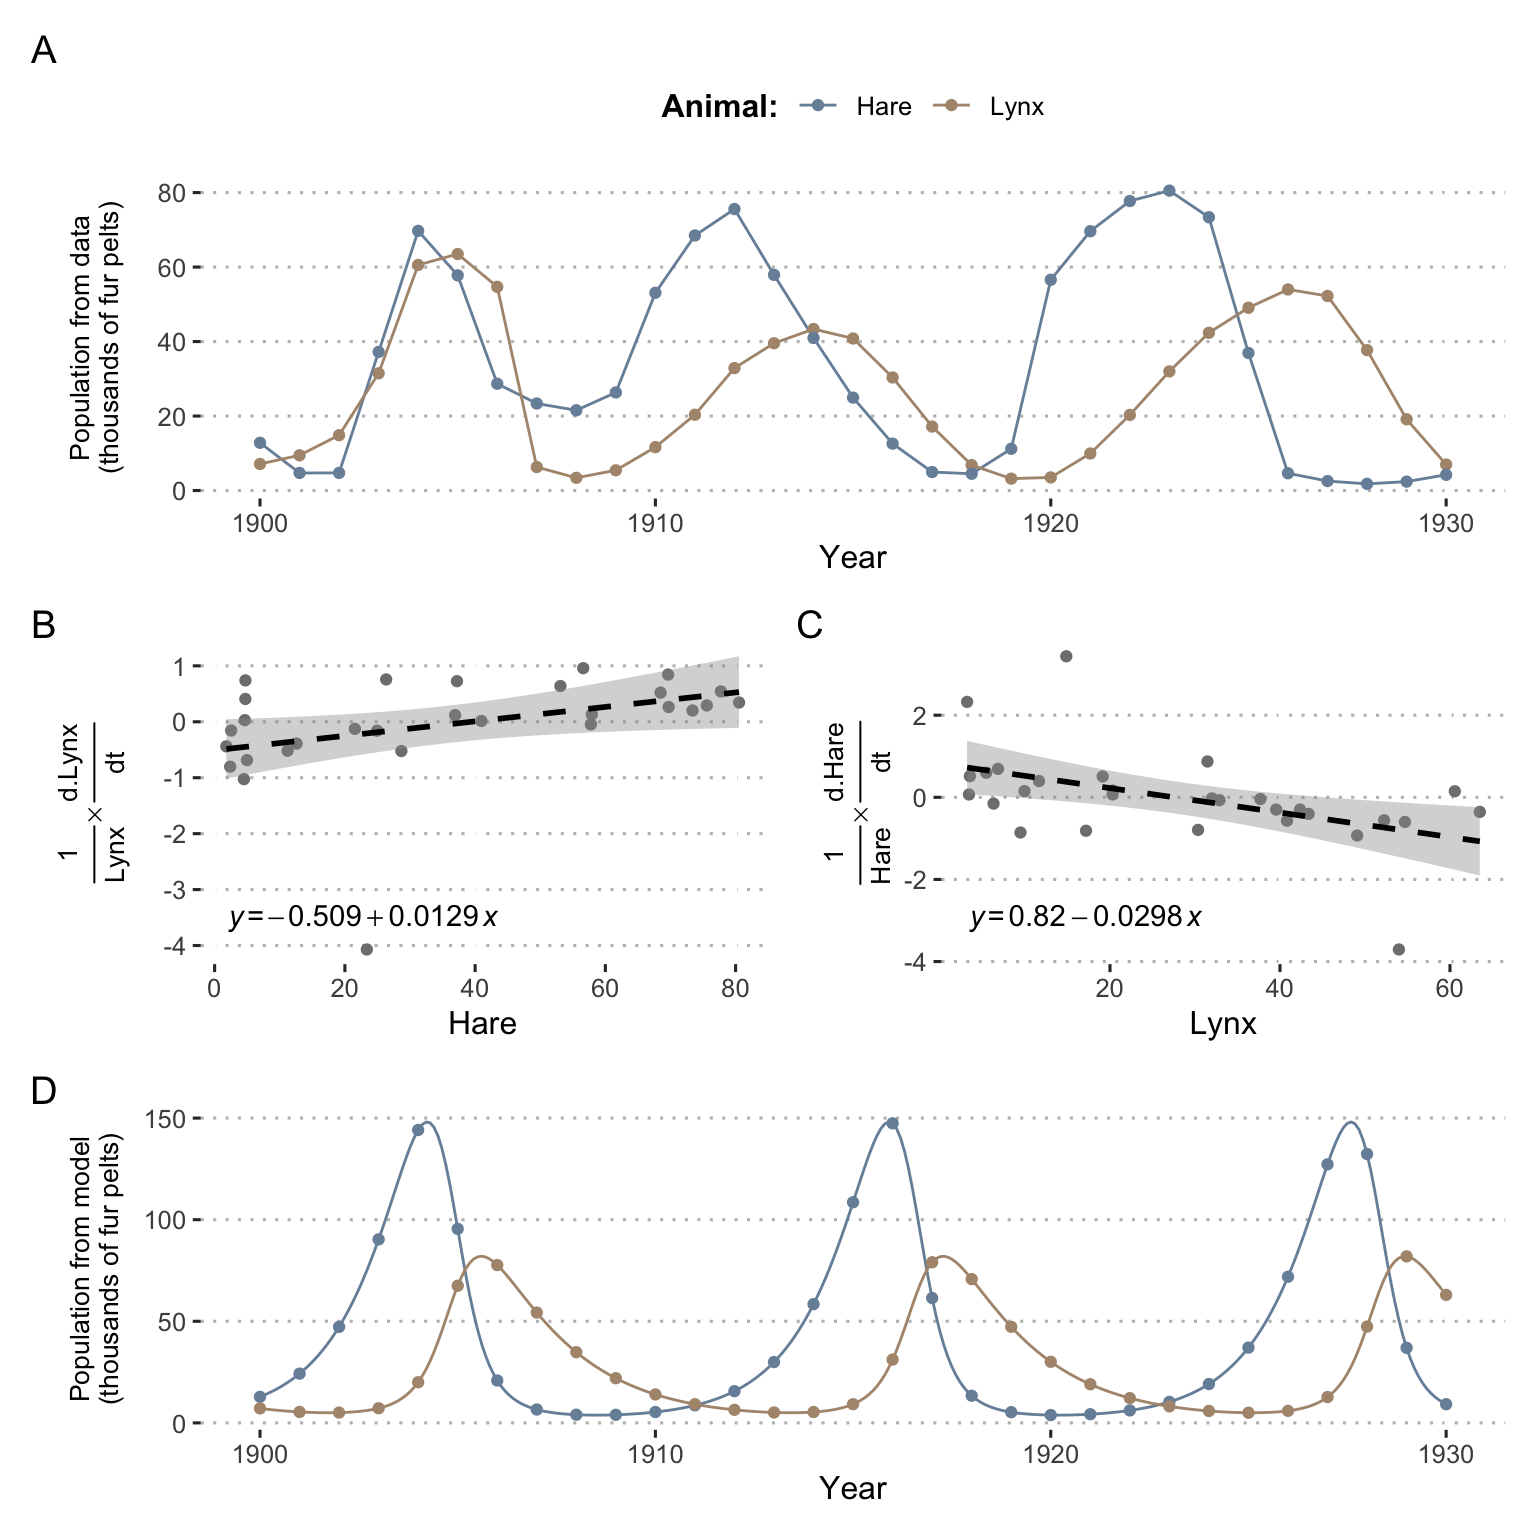
\includegraphics[width=0.9\linewidth]{01-Models_files/figure-latex/lotka-1} 

}

\caption[Some analyses around Lotka-Volterra model of a prey-predator system]{\textbf{Some analyses around Lotka-Volterra model of
a prey-predator system}. (A) Evolution of lynx and hares populations
based on Hudson Bay Company data about fur pelts. (B) and (C) Linear
regression for estimation of parameters. (D) Evolution of lynx and hare
populations as predicted by the model based on inferred parameters and
initial conditions.}\label{fig:lotka}
\end{figure}








This being said, the structure of the model having been defined a
priori, it remains to determine its parameters. Two options would
theoretically be possible: to propose values based on the interpretation
of the parameters and ecological knowledge, or to fit the model to the
data in order to find the best parameters. For the sake of simplicity,
and because this example has only a pedagogical value in this
presentation, we propose to determine them approximately using the
following Taylor-based approximation:

\[\dfrac{1}{y(t)} \dfrac{dy}{dt} \simeq \dfrac{1}{y(t)} \dfrac{y(t+1)-y(t-1)}{2}\]

By applying this approximation to the two equations of the differential
system and plotting the corresponding linear regressions (Figures
\ref{fig:lotka}B and C), we can obtain an evaluation of the parameters
such as \(a_1=0.82\), \(a_2=0.0298\), \(b_1=0.509\), \(b_2=0.0129\). By
matching the initial conditions to the data, the differential system can
then be fully determined and solved numerically (Figures
\ref{fig:lotka}D). Comparison of data and modeling provides a good
illustration of the virtues and weaknesses of a mechanistic model.
Firstly, based on explicit and interpretable hypotheses, the model was
able to recover the cyclical behaviour and dependencies between the two
species: the increase in the lynx population always seems to be preceded
by the increase in the hare population. However, the amplitude of the
oscillations and their periods are not exactly those observed in the
data. This may be related to approximations in the evaluation of
parameters, random variation in the data or, of course, simplifications
or errors in the structure of the model itself.

Besides, if one tries to carry out a statistical modeling of these data,
it is very likely that it is possible to approach the curve of
populations evolution much closer, especially for the hares. But should
it be expressed simply as a function of time or should a joint modeling
be proposed? The nature of the causal link between prey and predators
will be extremely difficult to establish without strong hypotheses such
as those of the mechanistic model. On the other hand, if populations in
later years had to be predicted as accurately as possible, it is likely
that a sufficiently well-trained statistical model would perform better.
Finally, and this is a fundamental difference, the \textbf{mechanistic
model enables to test cases or hypotheses that go beyond the scope of
the data}. Quite simply, by playing with the variables or parameters of
the model, we can predict the exponential decrease of predators in the
absence of prey and the exponential growth of prey in the absence of
prey. More generally, it is also possible to study analytically or
numerically the bifurcation points of the system in order to determine
the families of behaviours according to the relative values of the
parameters \citep{flake1998computational}. It is not possible to infer
these new or hypothetical behaviours directly from the data o of the
statistical model. This is theoretically possible on the basis of the
mechanistic model, provided that it is sufficiently relevant and that
its operating hypotheses cover the cases under investigation. Now that
the value of mechanistic models has been illustrated in a fairly
theoretical example, all that remains is to explore in the next chapters
how they can be built and used in the context of cancer.

\section{Simplicity is the ultimate
sophistication}\label{simplicity-is-the-ultimate-sophistication}

Before concluding this modeling introduction, it is important to
highlight one of the most important points already introduced in a
concise manner by the poet Paul Valéry at the beginning of this chapter.
\textbf{Whatever its nature, a model is always a simplified
representation of reality and by extension is always wrong to a certain
extent}. This is a generally well-accepted fact, but it is crucial to
understand the implications for the modeller. This simplification is not
a collateral effect but an intrinsic feature of any model:

\begin{quote}
\emph{No substantial part of the universe is so simple that it can be
grasped and controlled without abstraction. Abstraction consists in
replacing the part of the universe under consideration by a model of
similar but simpler structure. Models, formal and intellectual on the
one hand, or material on the other, are thus a central necessity of
scientific procedure.}\\
\citep{rosenblueth1945role}
\end{quote}

Therefore, a model exists only because we are not able to deal directly
with the phenomenon and simplification is a necessity to make it more
tractable \citep{potochnik2017idealization}. This simplification
appeared many times in the studies of frictionless planes or
theoretically isolated systems, in a totally deliberate strategy.
However, this idealization can be viewed in several ways
{[}weisberg2007three{]}. One of them, called Aristotelian or minimal
idealization, is to eliminate all the properties of an object that we
think are not relevant to the problem in question. This amounts to lying
by omission or making assumptions of insignificance by focusing on key
causal factors only \citep{frigg2020models}. We therefore refer to the
\emph{a priori} idea that we have of the phenomenon. The other
idealization, called Galilean, is to deliberately distort the theory to
make it tractable as explicited by Galileo himself:

\begin{quote}
\emph{We are trying to investigate what would happen to moveables very
diverse in weight, in a medium quite devoid of resistance, so that the
whole difference of speed existing between these moveables would have to
be referred to inequality of weight alone. Since we lack such a space,
let us (instead) observe what happens in the thinnest and least
resistant media, comparing this with what happens in others less thin
and more resistant.}
\end{quote}

This fairly pragmatic approach should make it possible to evolve
iteratively, reducing distortions as and when possible. This could
involve the addition of other species or human intervention into the
Lotka-Volterra system described above. A three-species Lotka-Volterra
model can however become chaotic \citep{flake1998computational}, and
therefore extremely difficult to use and interpret, thus underlining the
importance of simplifying the model.

We will have the opportunity to come back to the idealizations made in
the course of the cancer models but it is already possible to give some
orientations. The biologist who seeks to study cancer using cell lines
or animal models is clearly part of Galileo's lineage. The mathematical
or \emph{in silico} modeler has a more balanced profile. The design of
qualitative mechanistic models based on prior knowledge, which is the
core of the second part of the thesis, is more akin to minimal
idealization, which seeks to highlight the salient features of a system.
But the Galilean pragmatism consisting in creating
computationnaly-tractable models is also quite widespread, particularly
in highly dimensional statistical approaches.

Because of the complexity of the phenomena, simplification is therefore
a necessity. The objective then should not necessarily be to make the
model more complex, but to \textbf{match its level of simplification
with its assumptions and objectives}. Faced with the temptation of the
author of the model, or his reviewer, to always extend and complicate
the model, it could be replied with Lewis Carrol words\footnote{More
  concisely stated by \citet{rosenblueth1945role}: ``best material model
  for a cat is another cat, or preferably the same cat.''}:

\begin{quote}
\emph{``That's another thing we've learned from your Nation,'' said Mein
Herr, ``map-making. But we've carried it much further than you. What do
you consider the largest map that would be really useful?''}\\
\emph{``About six inches to the mile.''}\\
\emph{``Only six inches!'' exclaimed Mein Herr. ``We very soon got to
six yards to the mile. Then we tried a hundred yards to the mile. And
then came the grandest idea of all! We actually made a map of the
country, on the scale of a mile to the mile!''}\\
\emph{``Have you used it much?'' I enquired.}\\
\emph{``It has never been spread out, yet,'' said Mein Herr: ``the
farmers objected: they said it would cover the whole country, and shut
out the sunlight! So we now use the country itself, as its own map, and
I assure you it does nearly as well.''}\\
Lewis Carroll, \emph{Sylvie and Bruno} (1893)
\end{quote}

\chapter{Cancer as deregulation of complex
machinery}\label{cancer-as-deregulation-of-complex-machinery}

\epigraph{"All happy families are alike; each unhappy family is unhappy in its own way."}{Leo Tolstoy (Anna Karenina, 1877)}

\initial{A}rmed with all these models, whether statistical or
mechanistic, we are going to look at cancer, a particularly complex
system that fully justifies their use. Since the first chapter recalled
how important prior knowledge of the phenomenon under study is for
designing models, whatever their nature, this chapter will briefly
summarize some of the most important characteristics of this disease
before returning to the models themselves in the next chapter. Without
aiming for exhaustiveness, and after an epidemiological and statistical
description, we will focus on the most useful information for the
modeller, i.e.~the underlying biological mechanisms and available data.

\begin{figure}

{\centering 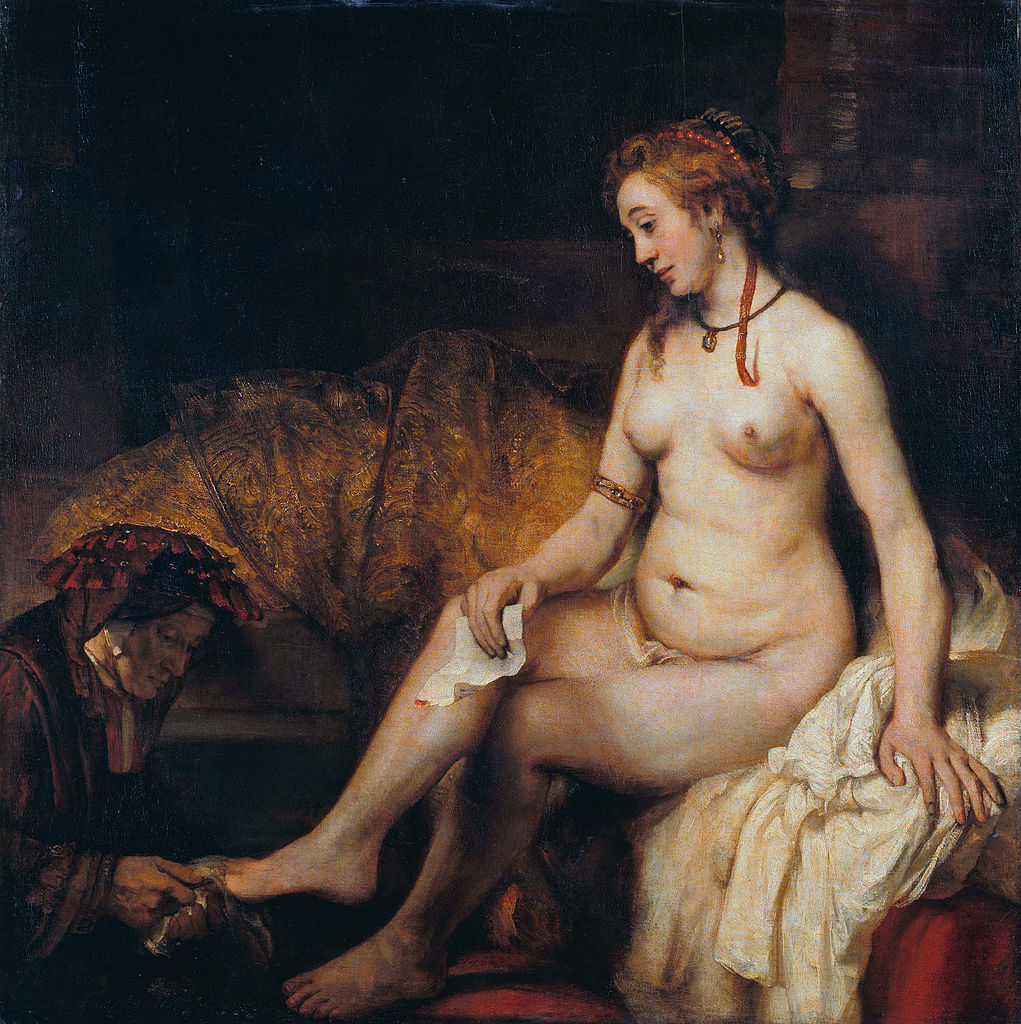
\includegraphics[width=0.9\linewidth]{fig/bath} 

}

\caption[Cancer is an old disease]{\textbf{Cancer is an old disease.} Rembrandt,
\emph{Bathsheba at Her Bath}, c. 1654, oil on canvas, Louvre Museum,
Paris}\label{fig:bath}
\end{figure}





\section{What is cancer?}\label{what-is-cancer}

Cancer can be described as a group of diseases characterized by
\textbf{uncontrolled cell divisions and growth which can spread to
surrounding tissues}. Descriptions of this disease, especially when
associated with solid tumours, have been found as far back as ancient
Egyptian documents, at least 1600 BC and we know from the first century
A.D. with Aulus Celsus that it is better to remove the tumors and this
as soon as possible \citep{hajdu2011note}. Progress will accelerate
during the Renaissance with the renewed interest in medicine, and
anatomy in particular, which will advance the knowledge of tumour
pathology and surgery \citep{hajdu2011note2}. The progress of anatomical
knowledge has also left brilliant testimonies in the field of painting,
which make the renown of the Renaissance today. The precision of these
artists' traits has also allowed some retrospective medical analyses,
some of them going so far as to identify the signs of a tumour in some
of the subjects of these paintings \citep{bianucci2018earliest}. Such is
the bluish stain on the left breast of the Bathsheba painted by
Rembrandt (Figure \ref{fig:bath}) which has been subject to
controversial interpretations, sometimes described as an example of
``skin discolouration, distortion of symmetry with axillary fullness and
peau d'orange'' \citep{braithwaite1983rembrandt} and sometimes spared by
photonic and computationnal analyses \citep{heijblom2014monte}. The
mechanisms of the disease only began to be elucidated with the
appearance of the microscope in the 19th century, which revealed its
cellular origin \citep{hajdu2012note}. The classification and
description of cancers is then gradually refined and the first
non-surgical treatments appear with the discovery of ionising radiation
by the Curies \citep{hajdu2012note2}. The 20th century is then the
century of understanding the causes of cancer
\citep{hajdu2013note, hajdu2013note2}. Some environmental exposures are
characterized as asbestos or tobacco. Finally, the biological mechanisms
become clearer with the identification of tumour-causing viruses and
especially with the discovery of DNA \citep{watson1953molecular}. The
foundations of our current understanding of cancer date back to this
period, which marks the beginning of the molecular biology of cancer. It
is this branch of biology that contains the bulk of the knowledge that
will be used to build our mechanistic models, and it will be later
detailed in Section \ref{molecular-biology}.

One of the ways to read this brief history of cancer is to see that
theoretical and clinical progress has not followed the same
timeframes.The medical and clinical management of cancers initially
progressed slowly but surely, and this in the absence of an
understanding of the mechanisms of cancer. Conversely, the theoretical
progress of the last century has not always led to parallel medical
progress, except on certain specific points. The interaction between the
two is therefore not always obvious. The \textbf{transformation of
fundamental knowledge into medical and clinical impact is therefore of
particular importance}. This is what is called \emph{translational
medicine}, the aim of which is to go from laboratory bench to bedside
\citep{cohrs2015translational}. It is in this perspective that we will
analyze the mechanistic models studied in this thesis. Their objective
is to integrate biological knowledge, or at least a synthesis this
knowledge, in order to transform it into a relevant clinical
information.

\section{Cancer from a distance: epidemiology and main
figures}\label{epidemio}

Before going down to the molecular level, it is important to detail some
figures and trends in the epidemiology of cancer today. Following the
description in the previous section, cancer is first and foremost
defined as a disease. Considered to be a unique disease, it caused 18.1
million new cancer cases and 9.6 million cancer deaths in 2018 according
to the Global Cancer Observatory affiliated to World Health Organization
\citep{bray2018global}. However, these aggregated data conceal
disparities of various kinds. The first one is geographical. Indeed,
mortality figures make cancer one of the leading causes of premature
death in most countries of the world but its importance relative to
other causes of death is even greater in the more developed countries
(Figure \ref{fig:globocan-map}). All in all, cancer is the first or
second cause of premature death in almost 100 countries worldwide
\citep{bray2018global}. These differences call for careful consideration
of the impact of population age structures and health-related
covariates.

\begin{figure}

{\centering 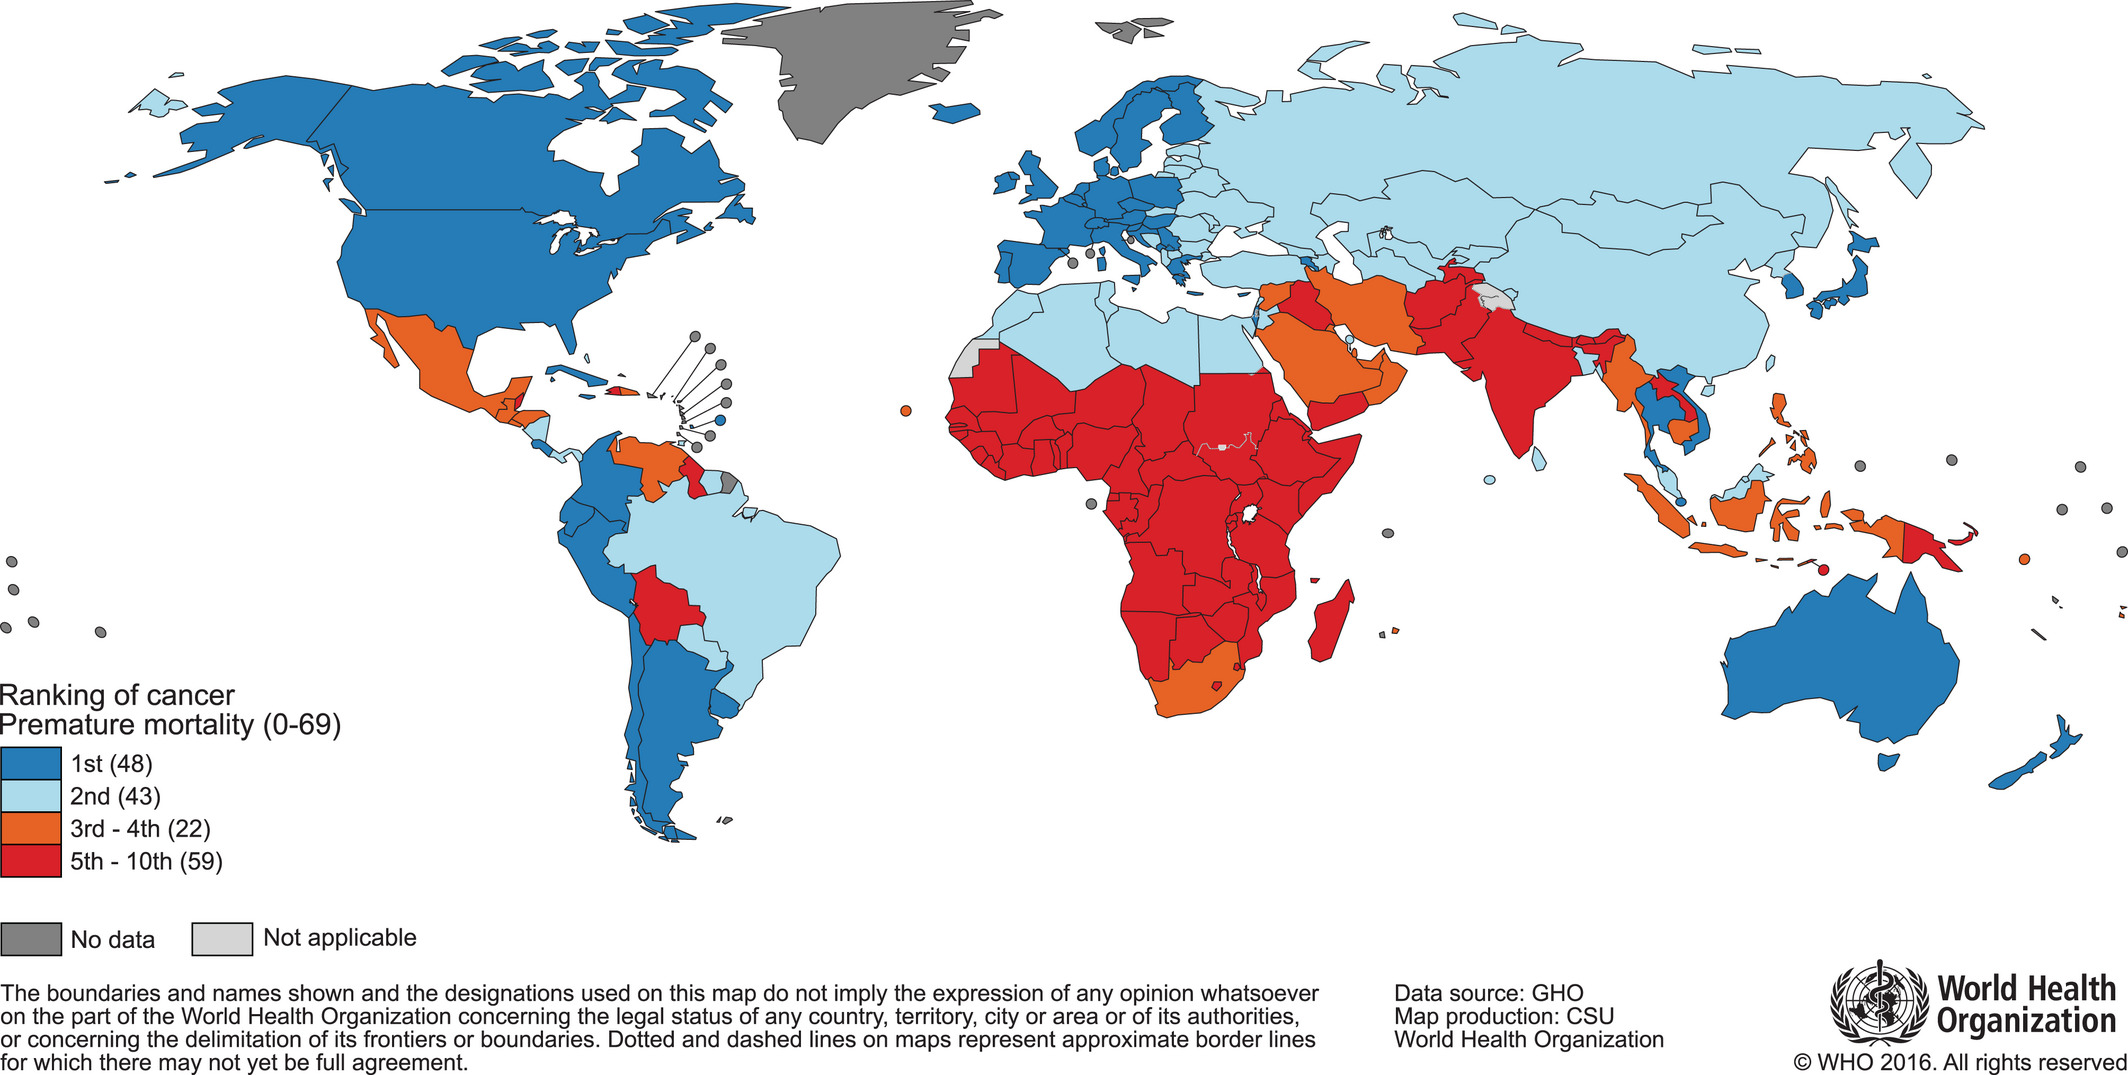
\includegraphics[width=0.9\linewidth]{fig/globocan-map} 

}

\caption[World map and national rankings of cancer as a cause of premature death]{\textbf{World map and national rankings of
cancer as a cause of premature death.} Classification of cancer as a
cause of death before the age of 70, based on data for the year 2015.
Original Figure, data and methods from \citet{bray2018global}.}\label{fig:globocan-map}
\end{figure}






A second disparity lies in the different types of cancer. If we classify
tumours solely according to their location, i.e.~the organ affected
first, we already obtain very wide differences. First of all, the
incidence varies considerably (Figure \ref{fig:cancer-tissues}A)).
Cancers do not occur randomly anywhere in the body and certain
environments or cell types appear to be more favourable
\citep{tomasetti2015variation}. Mortality is also highly variable but is
not directly inferred from incidence. Not all types of cancer have the
same prognosis (Figure \ref{fig:cancer-tissues}A and B) and survival
rates \citep{liu2018integrated}. Although breast cancer is much more
common than lung cancer, it causes fewer deaths because its prognosis
is, on average, much better. The mechanisms at work in the emergence of
cancer are therefore not necessarily the same as those that will govern
its evolution or its response to treatment. And still on the response to
treatment, Figure \ref{fig:cancer-tissues}B highlights another
disparity: not only are the survival prognosis associated with each
cancer very different, but the evolution (and generally the improvement)
of these prognoses has been very uneven over the last few decades. This
means that theoretical and therapeutic advances have not been applied to
all types of cancer with the same success. It is one more indication of
the \textbf{diversity of cancer mechanisms in different tissues and
biological contexts}, which make it impossible to find a panacea, and
which, on the contrary, encourage us to carefully consider the
particularities of each tumour, both to understand them and to treat
them. Under a generic name and in spite of common characteristics, the
cancers thus appear as extremely heterogeneous. And to understand the
sources of this heterogeneity, it is necessary to consider the disease
on a smaller scale.

\begin{figure}

{\centering 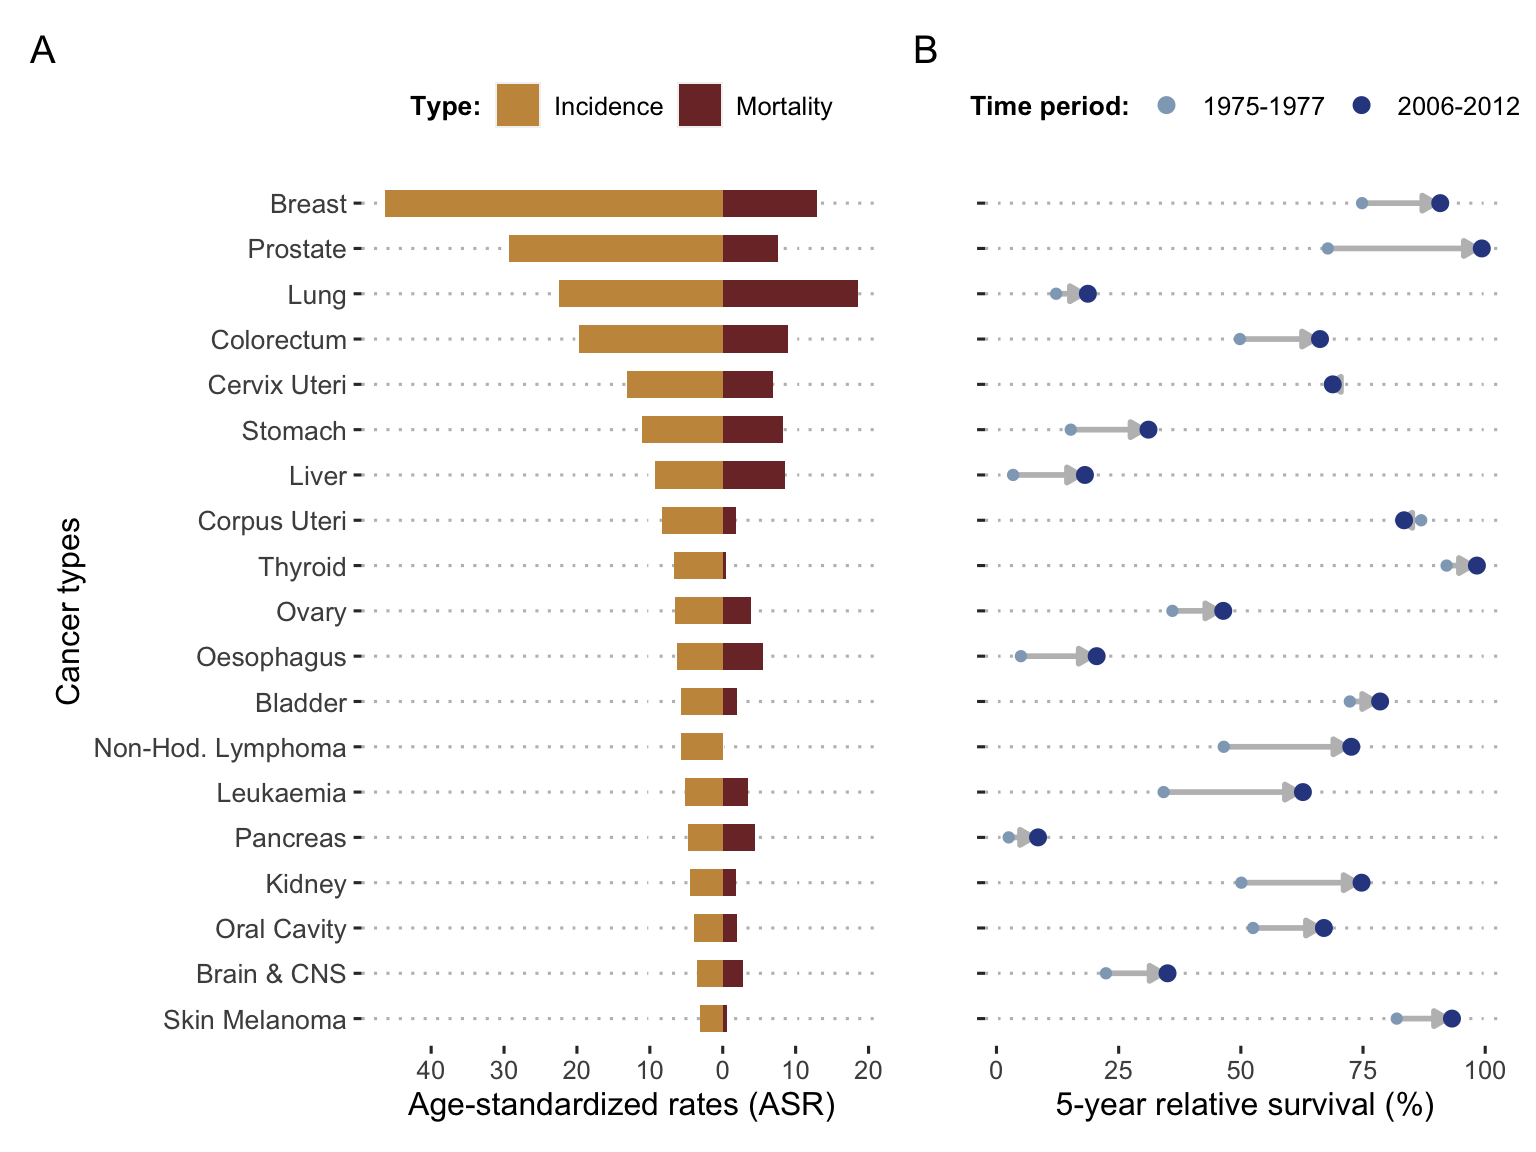
\includegraphics[width=0.9\linewidth]{02-Cancer_files/figure-latex/cancer-tissues-1} 

}

\caption[Incidence, mortality and survival per cancer types]{\textbf{Incidence, mortality and survival
per cancer types}. (A) World incidence and mortality for the 19 most
frequent cancer types in 2018, expressed with age-standardized rates
(adjusted age structure based on world population); data retrieved from
\href{https://gco.iarc.fr/today/home}{Global Cancer Observatory}. (B)
Evolution of 5-years relative survival for the same cancer types based
on US data from SEER registries in 1975-1977 and 2006-2012; data
retrieved from \citet{jemal2017annual}.}\label{fig:cancer-tissues}
\end{figure}










\section{Basic molecular biology and cancer}\label{molecular-biology}

If it is not possible and desirable to summarize here the state of
knowledge about the biology of cancer, we are going to give a very
partial vision focused on the main elements used in this thesis, thus
aiming to make it a self-sufficient document. The details necessary for
a finer and more general understanding can be found in dedicated
textbooks such as \citet{alberts2007molecular} and
\citet{weinberg2013biology}.

\subsection{Central dogma and core
principles}\label{central-dogma-and-core-principles}

Some of the principles that govern biology can be described at the level
of one of its simplest element, the cell. Let us consider for the moment
a perfectly healthy cell. It must ensure a certain number of functions
necessary for its survival and, if necessary, for its
division/reproduction. These functions are encoded in its genetic
information in the form of DNA, which is stable and shared by the
different cells since it is defined at the level of the individual. Most
biological functions, however, are not performed by DNA itself which
remains in the nucleus of the cell. The DNA is thus transcribed into
RNA, another nucleic acid which, in addition to performing some
biological functions, becomes the support of the genetic information in
the cell. The RNA is then itself translated into new molecules composed
of long chains of amino acid residues and called proteins. They are the
ones that execute most of the numerous cellular functions: DNA
replication, physical structuring of the cell, molecule transport within
the cell etc. A rather simplistic but fruitful way to understand this
functioning is to consider it as a \textbf{progressive transfer of
biological information from DNA to proteins}, which has sometimes been
summarized as the central dogma of the molecular biology
(\ref{fig:central-dogma}), first stated Francis Crick
\citep{crick1970central}.

\begin{figure}

{\centering 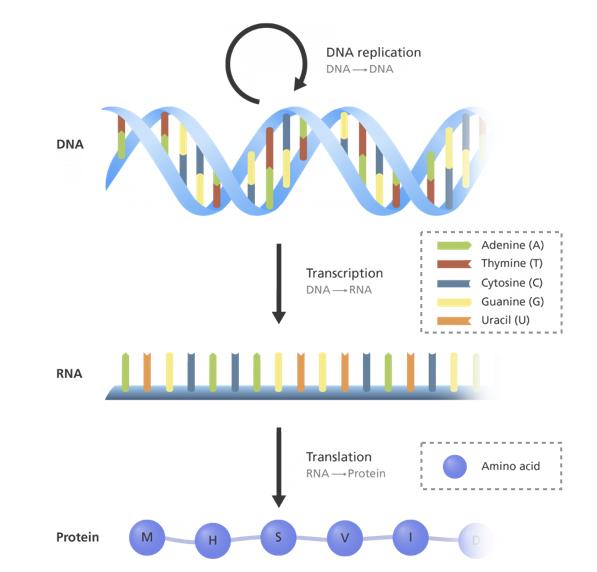
\includegraphics[width=0.8\linewidth]{fig/central-dogma} 

}

\caption[Central dogma of molecular biology]{\textbf{Central dogma of molecular biology.}
Schematic representation of the information flow within the cell, from
DNA to proteins through RNA, more precisely described in this
\href{https://www.youtube.com/watch?v=J3HVVi2k2No}{video} (Image credit
\emph{Genome Research Limited}).}\label{fig:central-dogma}
\end{figure}







However, many changes would be necessary to clarify this scheme and the
uni-directional nature was questioned early on. Above all, a large
number of regulations interact with and disrupt this master plan. The
genes are not always all transcribed, or at least not at constant
intensities, interrupting or varying the chain upstream. This modulation
in the transcription of genes can be induced by proteins, called
transcription factors. After a gene transcription, its expression can
still be regulated at various stages. RNAs can also be degraded more or
less rapidly. RNAs can be reshaped in their structure by a process
called splicing, which varies the genetic information they carry.
Finally, proteins are subject to all kinds of modifications referred to
as post-translational, which can change the chemical nature of certain
groups or modify the three-dimensional structure of the whole protein.
For instance, some proteins perform their function only if a specific
amino acid residue is phosphorylated. In addition, these modifications
can be transmitted between proteins, further complicating the flow of
information. \textbf{All these possibilities of regulation play an
absolutely essential role in the life of the cell by allowing it to
adapt to different contexts and situations}. From the same genetic
material, a cell of the eye and a cell of the heart can thus perform
different functions. Similarly, the same cell subjected to different
stimuli at different times can provide different responses because these
molecular stimuli trigger a regulation of its programme. But all these
regulatory mechanisms can be corrupted.

\subsection{A rogue machinery}\label{a-rogue-machinery}

With the above knowledge we can now return to the definition of cancer
as an uncontrolled division of cells that can lead to the growth of a
tumour that eventually spreads to the surrounding tissues. Therefore,
this corresponds to normal processes, like cell division and
reproduction, that are no longer regulated as they should be and are out
of control. Experiments on different model organisms have gradually
identified genetic mutations as a major source of these deregulations
\citep[\citet{reddy1982point}]{nowell1976clonal} until cancer was
clearly considered as a \textbf{genetic disease} making Renato Dulbecco,
Nobel Laureate in Medicine for his work on oncoviruses, say:

\begin{quote}
\emph{If we wish to learn more about cancer, we must now concentrate on
the cellular genome.}\\
\citep{dulbecco1986turning}.
\end{quote}

However, cancer is not a Mendelian disease for which it would be
sufficient to identify the one and only gene responsible for
deregulation. Indeed, the cell has many protective mechanisms. For
example, if a genetic mutation appears in the DNA, it has a very high
chance of being repaired by dedicated mechanisms. And if it is not
repaired, other mechanisms will take over to trigger the programmed
death of the cell, called apoptosis, before it can proliferate wildly.
So a cancer cell is probably a cell that has learned to resist this cell
death. Similarly, in order to generate excessive growth, a cell will
need to be able to replicate itself many times. However, there are
pieces of sequences on chromosomes called telomeres that help to limit
the number of times each cell can replicate. A cancer cell will
therefore have to manage to bypass this protection. Thus we can
schematically define the properties that must be acquired by the
cancereous cells in order to truly deviate the machinery. In an
influential article, these properties were summarized in six hallmarks
(Figure \ref{fig:hallmarks}) which are: resisting cell death, enabling
replicatve immortality, sustaning proliferative signaling, evading
growth suppressors, activating invasion and inducing angiogenesis
\citep{hanahan2000hallmarks}. Two new ones were subsequently added in
the light of advances in knowledge \citep{hanahan2011hallmarks}:
deregulating cancer energetics and avoiding immne destruction. The
acquisition of these capacities generally requires many genetic
mutations and is therefore favoured by an underlying genome instability.

\begin{figure}

{\centering 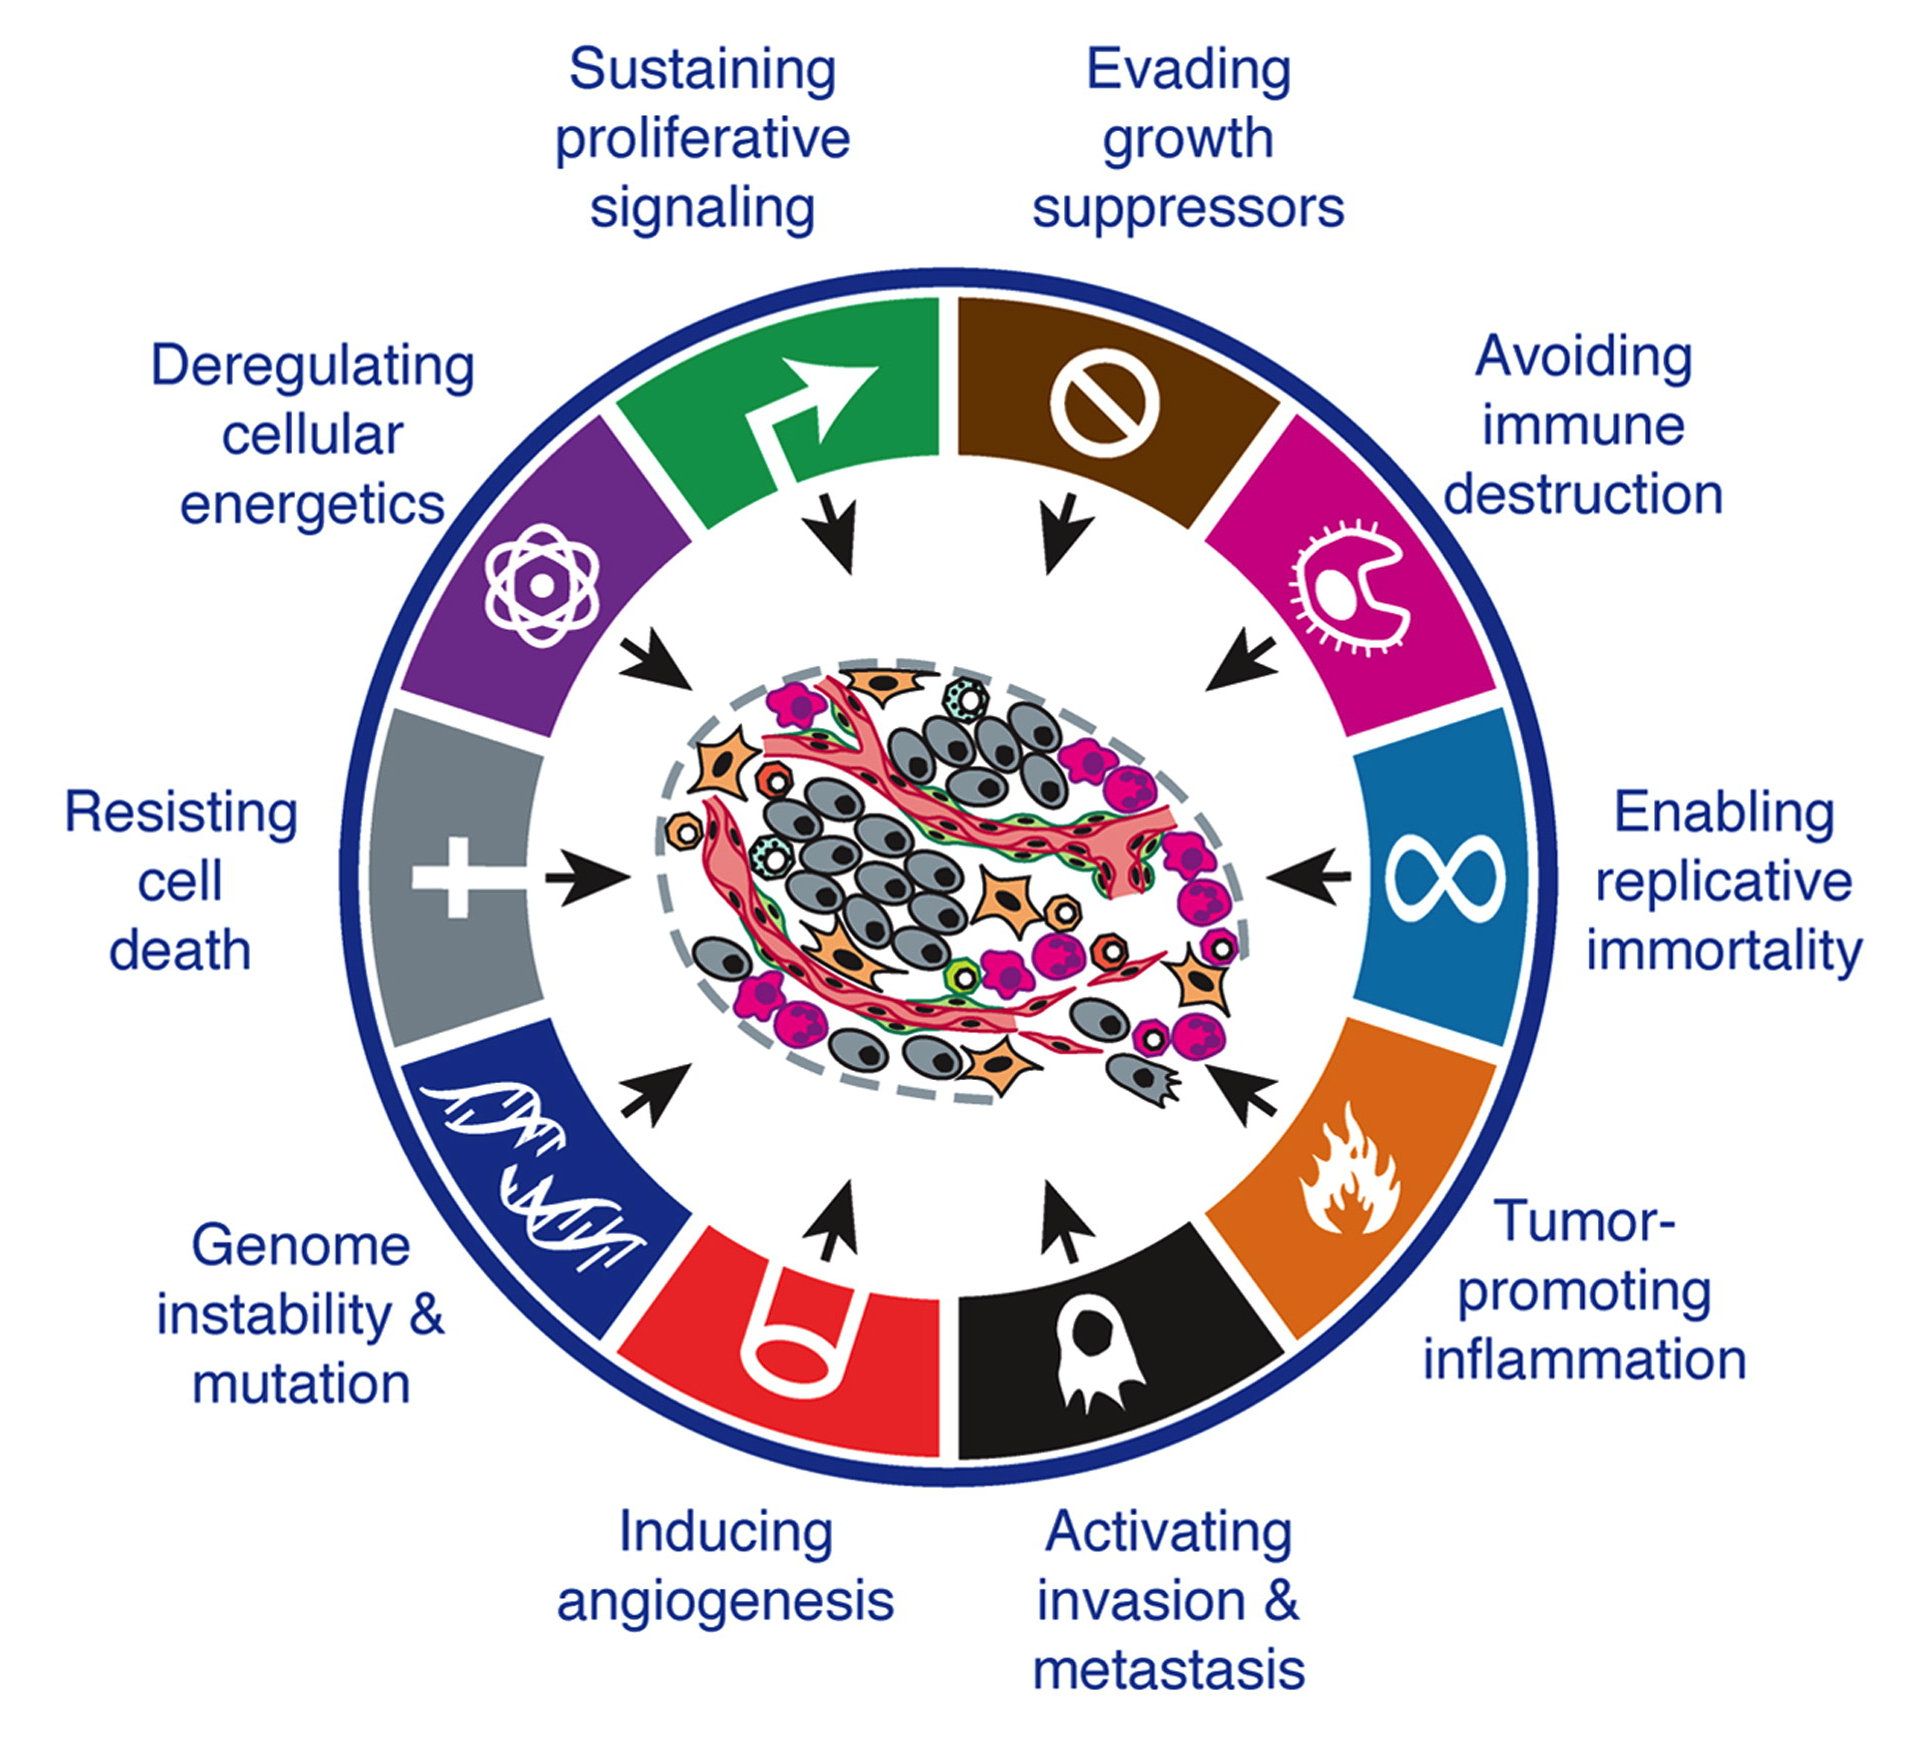
\includegraphics[width=0.9\linewidth]{fig/hallmarks} 

}

\caption[Hallmarks of cancer]{\textbf{Hallmarks of cancer.} The different
biological capabilities acquired by cancer cells, as described in
\citet{hanahan2000hallmarks}. Reprinted from
\citet{hanahan2011hallmarks}.}\label{fig:hallmarks}
\end{figure}






Each of these characteristics, or hallmarks, constitutes a research
program in its own right. And for each one there are genetic
alterations. These are tissue-specific or not, specific to a hallmark or
common to several of them \citep{hanahan2000hallmarks}. In any case,
\textbf{cancer can only result from the combination of different
alterations that invalidate several protective mechanisms} at the same
time. This is often part of a multi-step process of hallmark acquisition
that has been experimentally documented in some specific cases
\citep{hahn1999creation} or more recently inferred from genome-wide data
for human patients \citep{tomasetti2015only}. In summary, it appears
that in order to study the functioning of cancer cells it is necessary
to look at several mechanisms and to be able to consider them not
separately but together, in as many different patients as possible. This
ambitious programme has been made possible by a technological
revolution.

\section{The new era of genomics}\label{the-new-era-of-genomics}

\subsection{From sequencing to multi-omics
data}\label{from-sequencing-to-multi-omics-data}

In 2001, the first sequencing of the human genome symbolized the
beginning of a new era, that of what will become \textbf{high-throughput
genomics} \citep{lander2001initial, venter2001sequence}. From the end of
the 20th century, biological data started to accumulate at an
ever-increasing rate \citep{reuter2015high}, feeding and accelerating
cancer research in particular
\citep{stratton2009cancer, meyerson2010advances}. The ability to
sequence the human genome as a whole, for an ever-increasing number of
individuals, has enabled \textbf{less biased and more systematic studies
of the causes of cancer} \citep{lander2011initial}. The number of genes
associated with cancer increased drastically and some very important
genes such as BRAF of PIK3CA have been identified
\citep{davies2002mutations, samuels2004high}. Progress also extended to
the gene expression data. Gene-expression arrays have made an important
contribution by providing access to transcriptomic data (RNA), i.e.~what
has been transcribed from DNA and is therefore one step further in terms
of biological information. This information has made it possible to
further explore the differences betwween normal and tumour cells
\citep{perou1999distinctive}, or even to refine the classification of
cancers, which until now has been done mainly according to the tumour
site. Breast cancers are thus divided into subtypes with different
combinations of molecular markers that facilitate the understanding of
clinical behavior \citep{perou2000molecular}. One step further, we also
note the appearance of prognostic gene signatures such as gene
expression patterns correlated with the survival of patients
\citep{van2002gene}. This revolution was then extended to other types of
data such as proteins (proteomics), reversible modifications of DNA or
DNA-associated proteins (epigenomics), metabolites (metabolomics) and
others, each representing a perspective that can complement the others
to better understand biological mechanisms, particularly in the case of
diseases \citep{hasin2017multi}. We have thus entered the era of
multi-omics data \citep{vucic2012translating}.

\subsection{State-of-the art of cancer
data}\label{state-of-the-art-of-cancer-data}

With respect to cancer in particular, this wealth of data is
particularly represented by a family of \textbf{studies conducted by The
Cancer Genome Atlas (TCGA) consortium}, started in 2008
\citep{cancer2008comprehensive}. Cohorts of several hundred patients are
thus sequenced over the years for different types of cancer
\citep{cancer2012comprehensive}, resulting today in a total of 11,000
tumors from 33 of the most prevalent forms of cancer
\citep{ding2018perspective}. Figure \ref{fig:tcga} provides a partial
but striking overview of the depth of data available under this program.
We can see the frequencies of alterations of certain groups of genes for
a list of cancer types, making it possible to visualize the disparities
already anticipated in section \ref{epidemio} based on patient survival.
There are indeed important differences between the organs but also
between the different subtypes associated with the same organ. And this
representation only corresponds to one layer of data, that of genetic
alterations. It could be used for transcriptomic, epigenomic or
proteomic data, thus giving rise to an incredibly complex photography.

\begin{figure}

{\centering 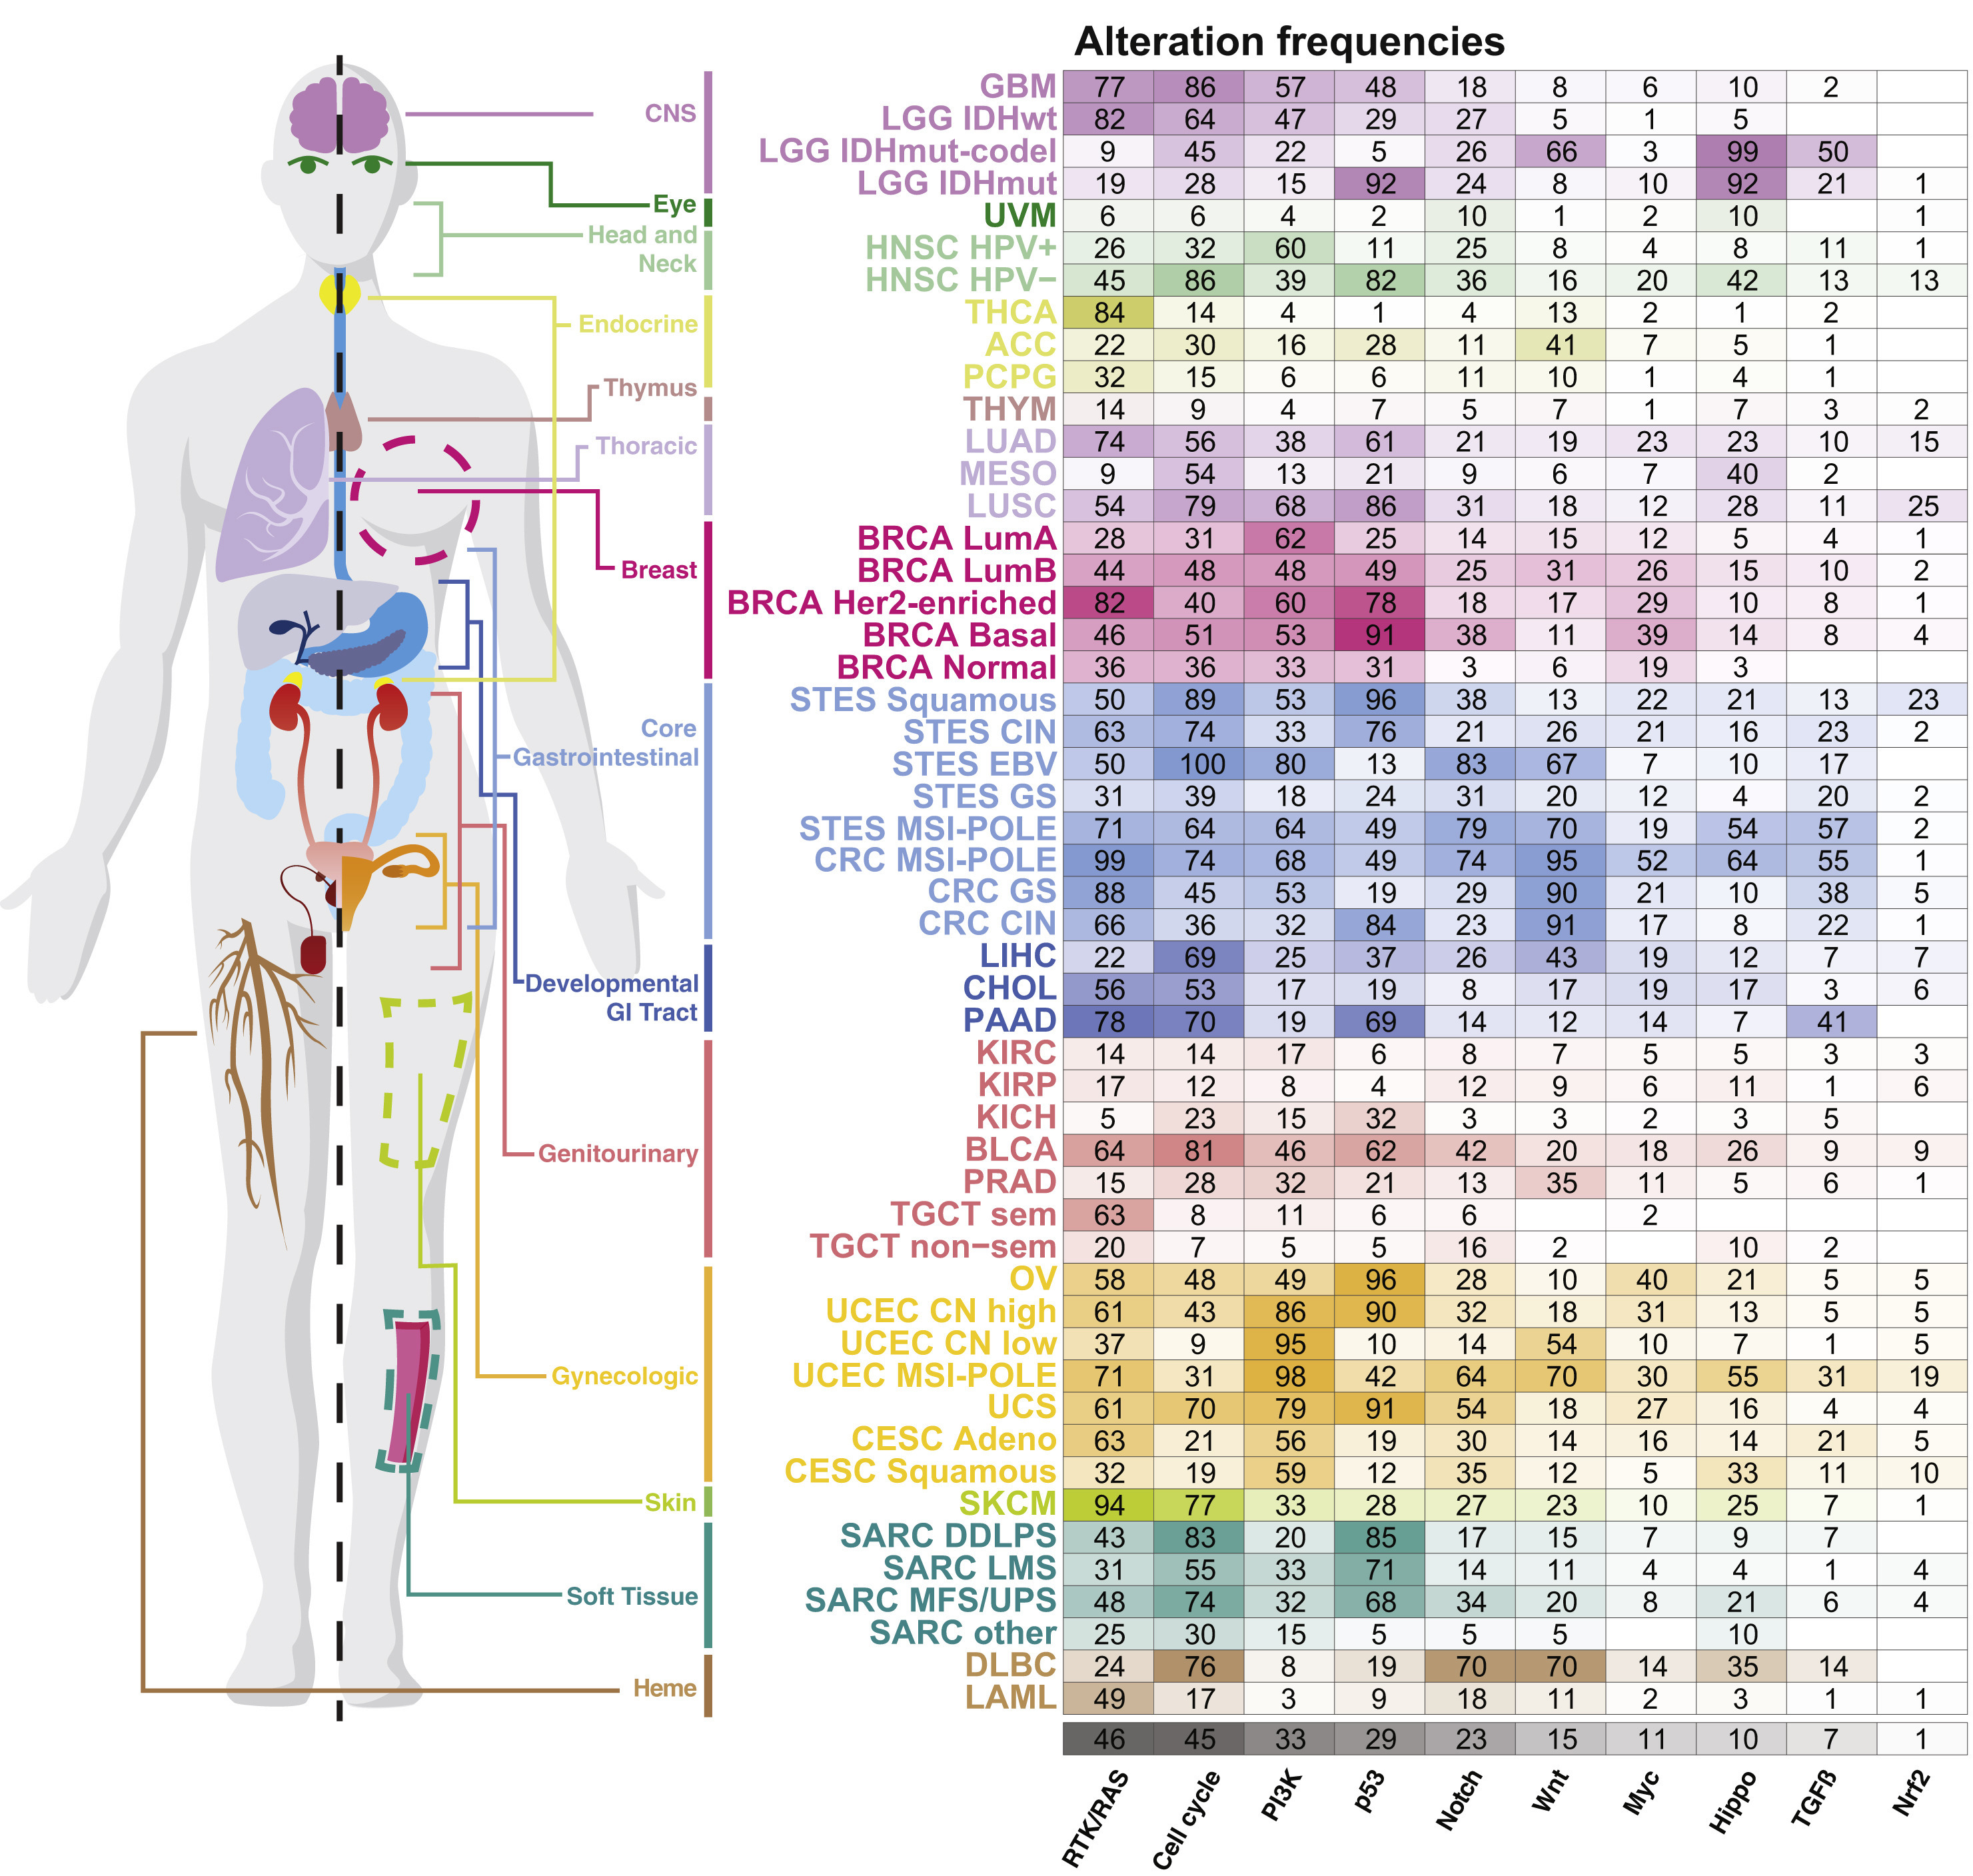
\includegraphics[width=0.9\linewidth]{fig/tcga} 

}

\caption[Genetic alterations frequencies for cancer types from TCGA data]{\textbf{Genetic alterations frequencies for cancer
types from TCGA data.} Frequencies of alteration per pahway and tumour
types as summaried in Pan-cancer analyses from TCGA data. Reprinted from
\citet{sanchez2018oncogenic}.}\label{fig:tcga}
\end{figure}






However, the diversity of data available for cancer research extends far
beyond this, both in terms of technology and type of data. This may be
data from model organisms such as mice or tumours of human origin made
more suitable for experimentation. In the latter category, it is crucial
to mention the \textbf{huge amount of data available on cell lines},
extracted from human tumours and transformed to be studied in culture.
It is then possible to go beyond descriptive data and vary the
experimental conditions in order to study the responses of these cells
to perturbations and to enrich our knowledge. This provides an
opportunity to know the response to more than 100 drugs of about 700
cell lines \citep{yang2012genomics}. The richness of these data, coupled
with the omic profiling of each cell line, enables to study the
determinants of response to treatment with unprecedented scope
\citep{iorio2016landscape}. More recently, but following a similar
logic, other types of inhibition screenings have been proposed based on
a more specific technique called CRISPR-Cas9
\citep{behan2019prioritization}. The simplicity of the cell lines in
relation to the original tumours makes all these studies possible but
sometimes hinders the clinical application of the knowledge acquired.
For this reason, other types of biological models have been developed,
including patient-derived xenografts (PDX) which is an implant of human
tumours in mice to maintain the existence of a certain tumour
microenvironment \citep{hidalgo2014patient}, while maintaining drug
screening possibilities \citep{gao2015high}. These two types of data,
cell lines and PDX, have been used in this thesis, in addition to TCGA
patient data, thus justifying the limitation of this presentation, which
could otherwise be extended to other types of biological models.
Similarly, other technologies are becoming increasingly important in the
generation of cancer data, such as single-cell sequencing
\citep{navin2015first}, but will not be used in this work.

\section{Data and beyond: from genetic to network
disease}\label{data-and-beyond-from-genetic-to-network-disease}

All that remains to be done now is to make sense of all these data, to
organize it, because \textbf{cancer understanding does not flow directly
from the abundance of data}, and the ability to produce it may have been
outpaced by the ability to analyze it \citep{stadler2014cancer}. A
striking example is that of the prognostic signatures mentioned above.
The many signatures or lists of genes proposed, even for the same cancer
type, share relatively few genes, are difficult to interpret and their
efficiency is sometimes poorly reproducible \citep{domany2014using}.
Even more surprisingly, most signatures composed of randomly selected
genes were also found to be associated with patient survival
\citep{venet2011most}. One of the main avenues for improving the
interpretability of the data is the \textbf{integration of the prior
knowledge} we have of the phenomena, especially in the case of cancer
\citep{domany2014using}.

\begin{figure}

{\centering 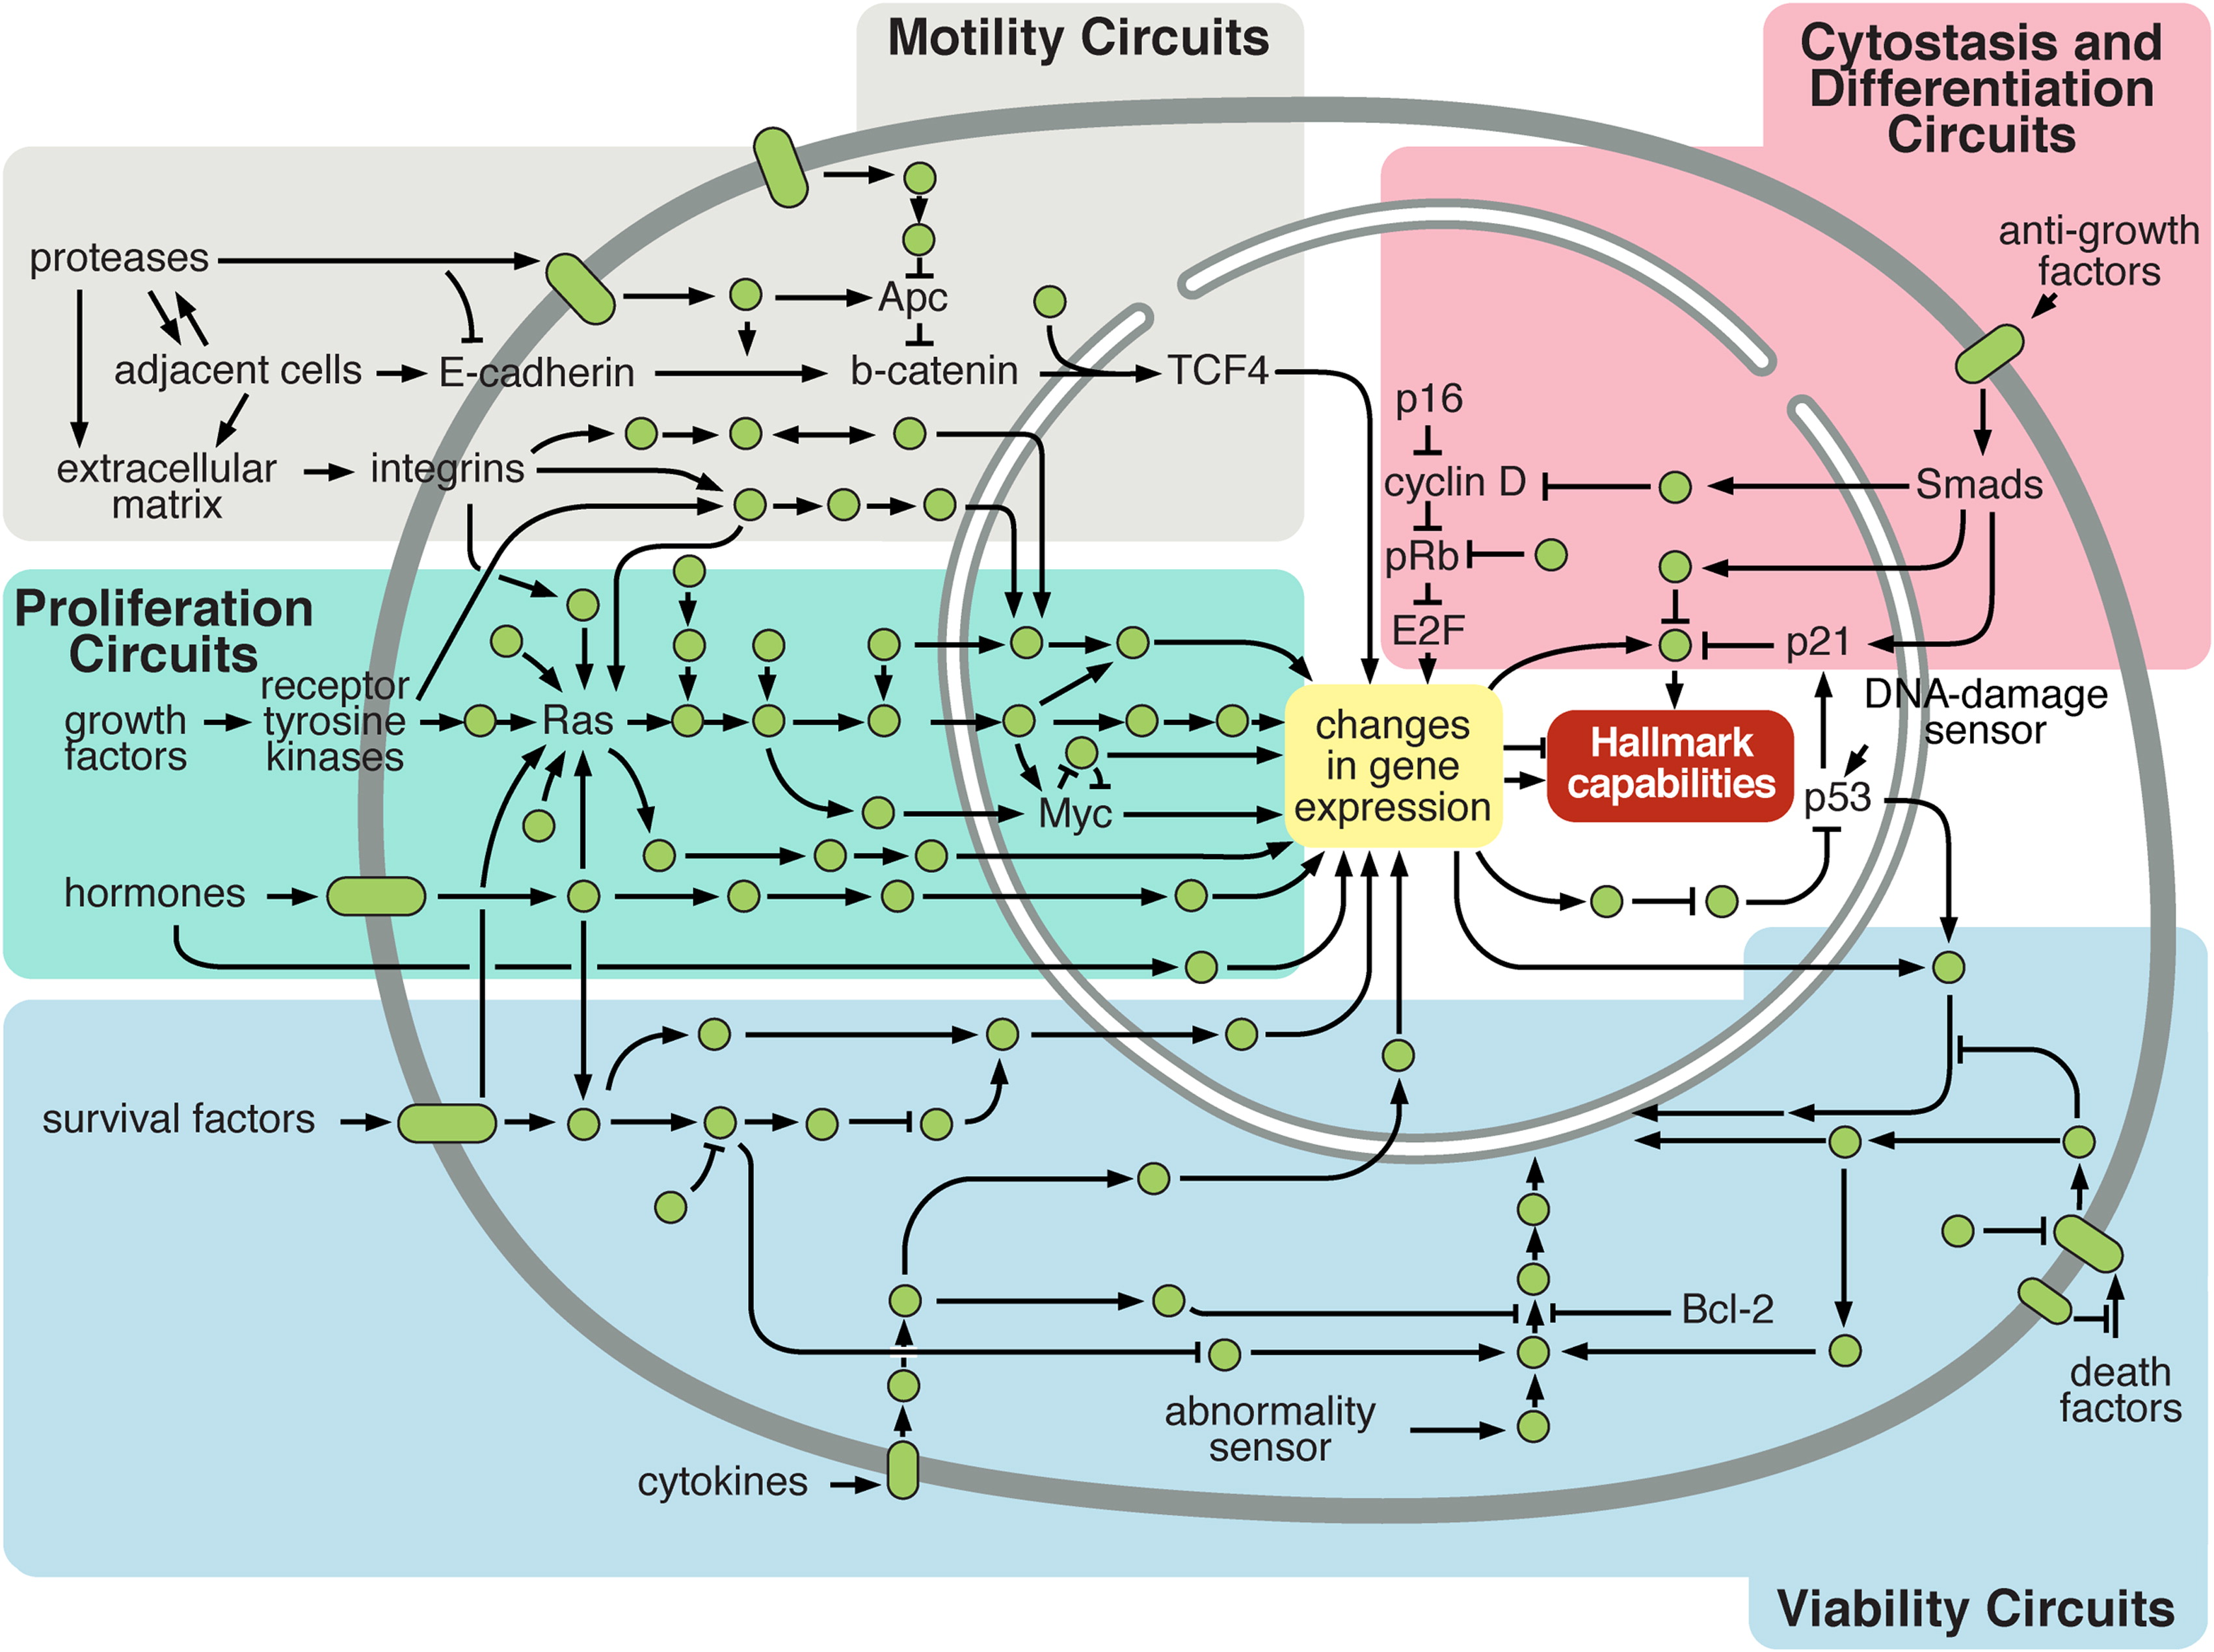
\includegraphics[width=0.9\linewidth]{fig/circuit} 

}

\caption[Simplistic representation of cellular circuit and pathways]{\textbf{Simplistic representation of cellular
circuitry.} Normal cellular circuit sand sub-circuits (identified by
colours) can be reprogrammed to regulate hallmark capabilities within
cancer cells. Reprinted from \citet{hanahan2011hallmarks}.}\label{fig:circuit}
\end{figure}






This \emph{a priori} knowledge is in fact already present in Figure
\ref{fig:tcga} since genetic alterations have been grouped in several
categories called pathways. A pathway is group of biological entities,
and associated chemical reactions, working together to control a
specific cell function like apoptosis or cell division. The interest of
these groupings may be understood based on the description of hallmarks.
Indeed, if the ``aim'' of a cancer cell is to inactivate each of the
protective functions, then it is more relevant to think not by gene but
by function. Inactivating only one of the genes associated with the
function may be sufficient and it is no longer necessary to inactivate
the others. Numerous alterations in a large number of genes in various
patients result often in the same key impaired pathways, like
alterations of cell cycle or angiogenesis for instance
\citep{jones2008core}. It is therefore possible to improve the stability
and interpretability of analyses by moving \textbf{from the gene scale
to the pathway scale} \citep{drier2013pathway}. More generally, the
integration of biological knowledge often leads to improved performance
in various cancer-related prediction tasks, either through the selection
of variables or by taking into account the structure of the variables
\citep{bilal2013improving, ferranti2017value}. Increasingly, the
biological variables are not interpreted separately but in relation to
each other \citep{barabasi2004network}. This is reflected in the
emergence of more and more resources to summarize and represent
signaling pathways and associated networks such as SIGNOR
\citep{perfetto2016signor}, OmniPath \citep{turei2016omnipath} or the
Atlas of Cancer Signaling Network \citep{kuperstein2015atlas}. Like
other diseases, cancer then goes \textbf{from a genetic disease to a
network disease} \citep{del2010diseases} and one can study how all kinds
of genetic alterations affect the wiring of these networks
\citep{pawson2007oncogenic}, and modify the cellular functions leading
to the previously described cancer hallmarks as depicted schmatically in
Figure \ref{fig:circuit}. In short, the richness of the data did not
make it less necessary to use prior knowledge in order to make the
analyses more interpretable and more robust.

\begin{figure}

{\centering 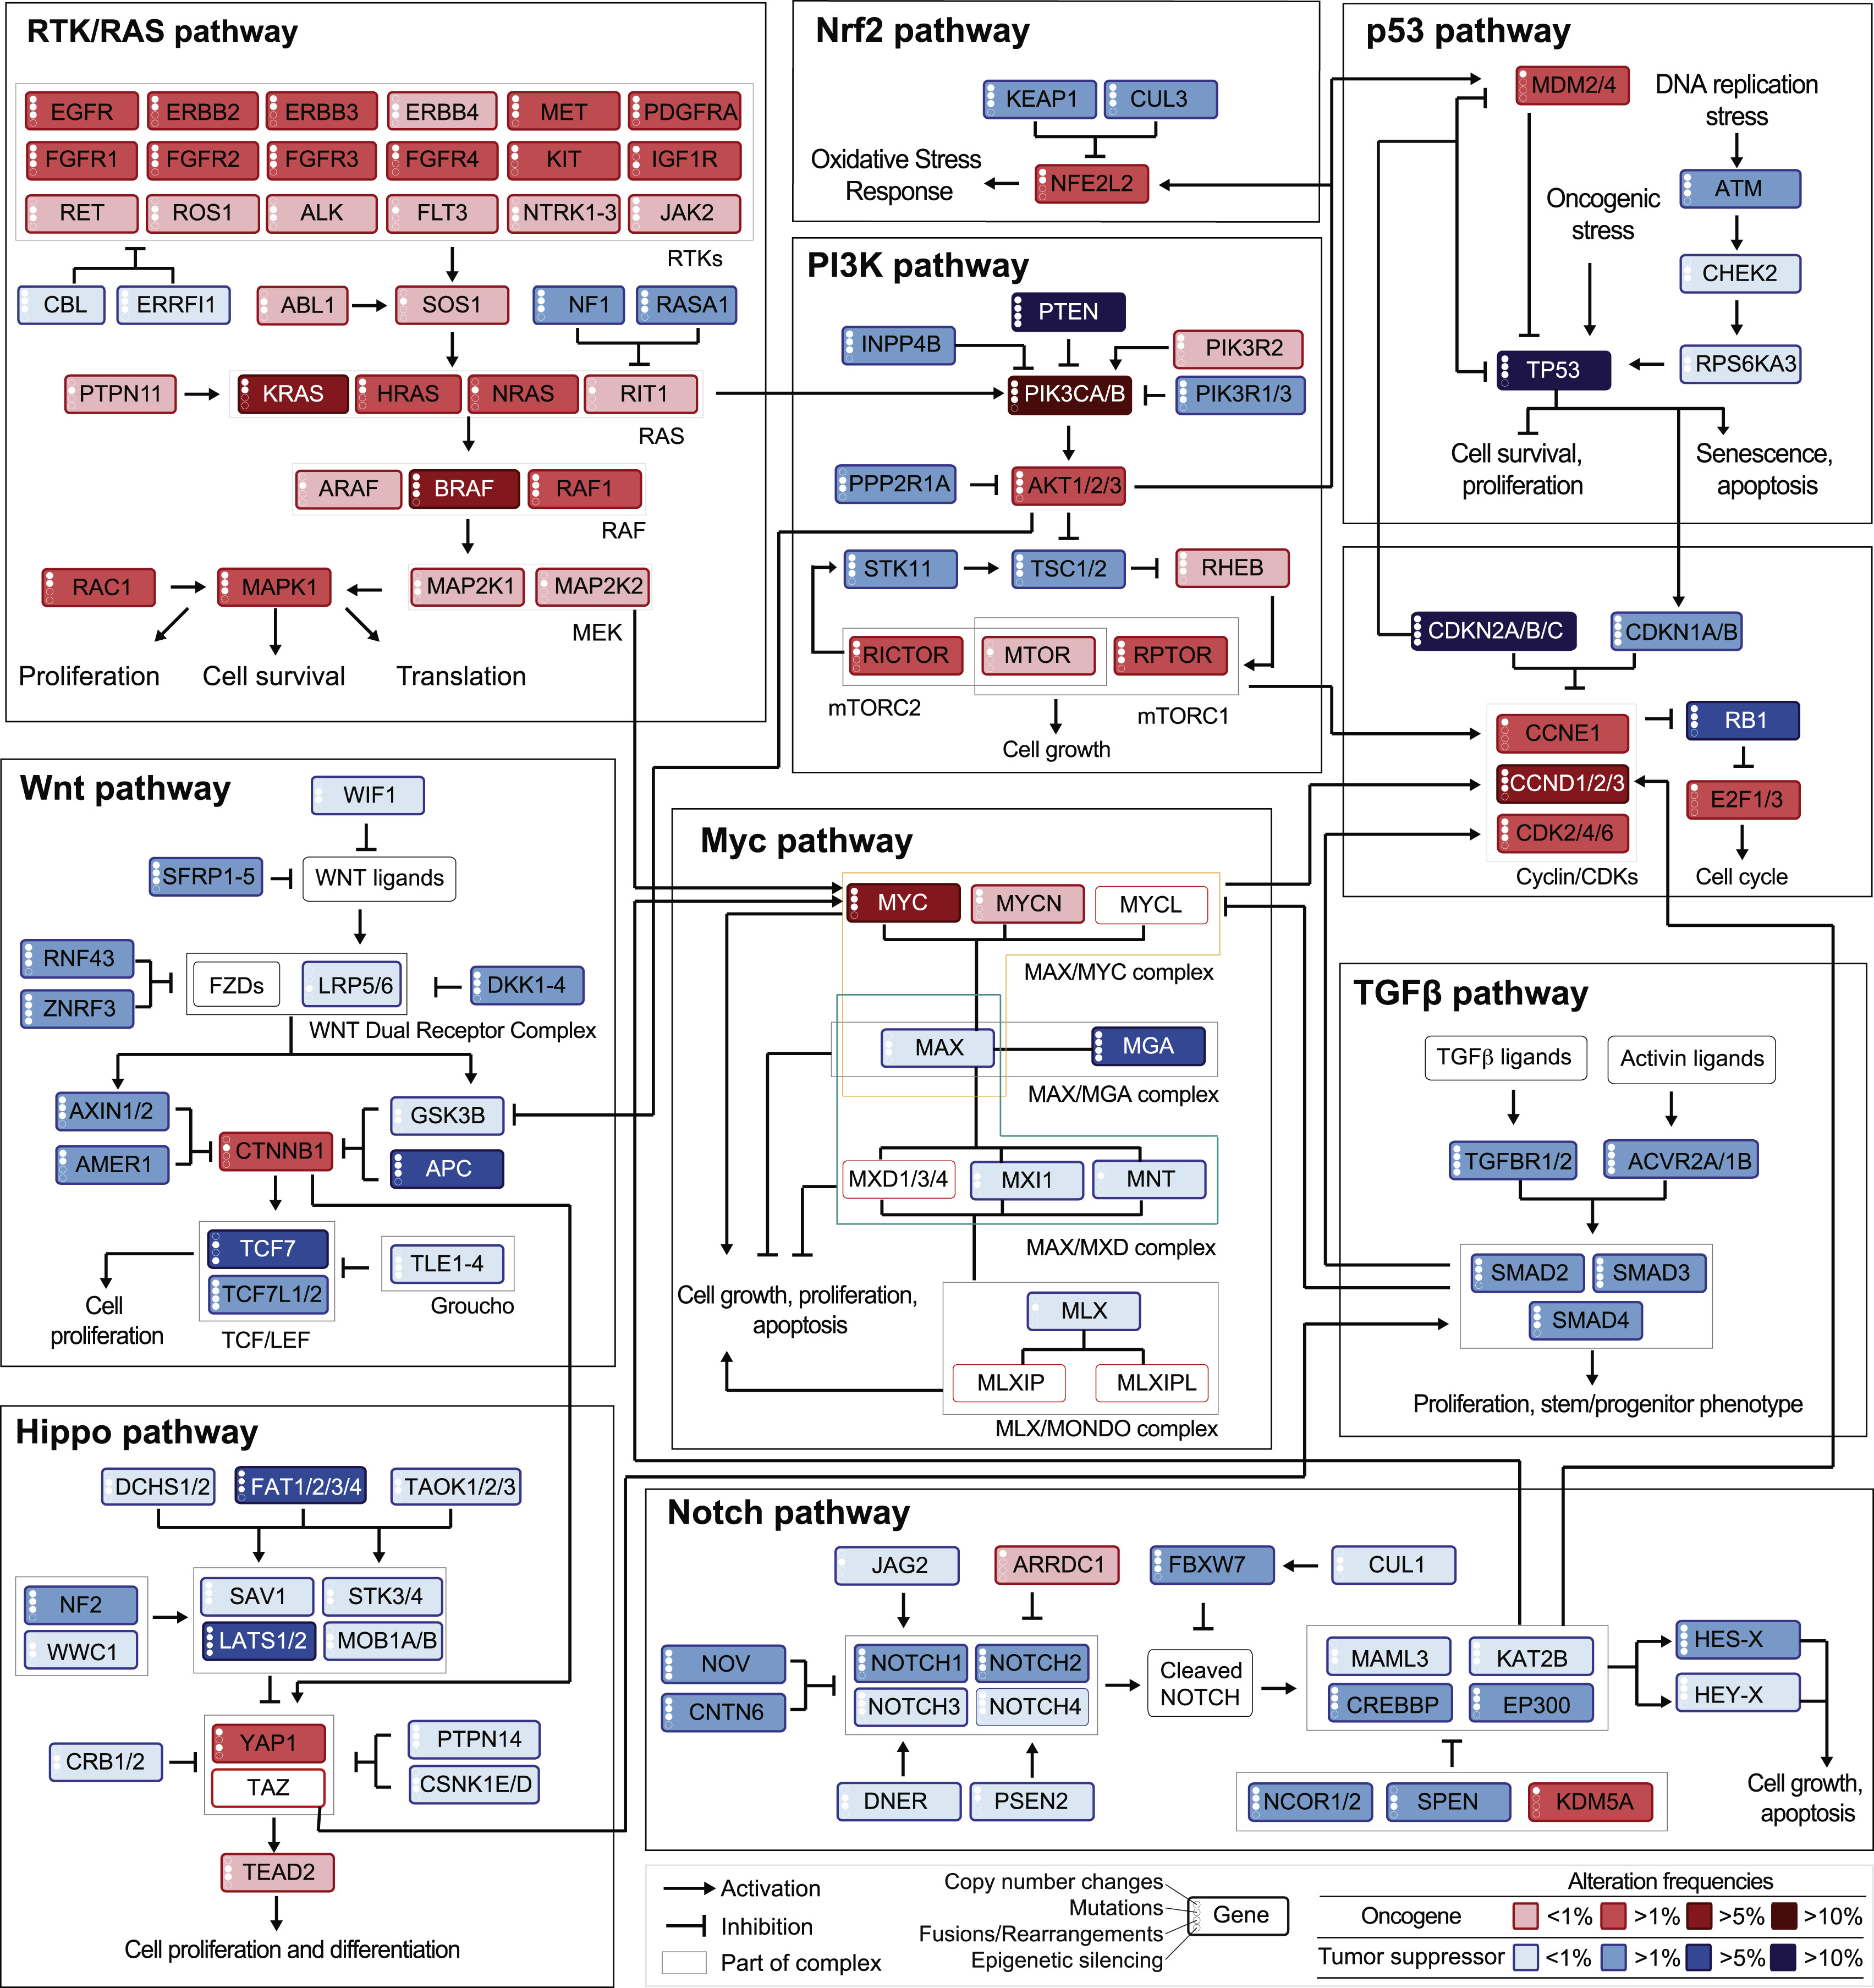
\includegraphics[width=0.9\linewidth]{fig/pathways} 

}

\caption[Genetic alterations frequencies from TCGA data mapped on a schematic signaling network]{\textbf{Genetic alterations frequencies from TCGA
data mapped on a schematic signaling network.} Frequencies of alteration
per pathway and tumour types as summarized in Pan-cancer analyses from
TCGA data. Reprinted from \citet{sanchez2018oncogenic}.}\label{fig:pathways}
\end{figure}






The final step, to obtain one of the most complete and integrated
visions of cancer biology, is then to integrate omics knowledge with
knowledge about the structure of pathways to try to understand in detail
how their combinations can lead to so many cancers that are both similar
and different. An example of such a representation is given by mapping
the TCGA data about genetic alterations, presented in Figure
\ref{fig:tcga}, on a representation of the different pathways showing
not only their internal organization but also their cross-talk
\citep{sanchez2018oncogenic}. This representation is proposed in Figure
\ref{fig:pathways} and is one the most recent and comprehensive view of
the kind of tools and data available to the modeller who wants to
dissect more deeply the mechanisms involved in cancer.

\chapter{Mechanistic modeling of cancer: from complex disease to systems
biology}\label{mechanistic-cancer}

\epigraph{"How remarkable is life? The answer is: very. Those of us who deal in networks of chemical reactions know of nothing like it... How could a chemical sludge become a rose, even with billions of years to try."}{George Whitesides}

\initial{T}he previous chapter identified the need to organize cancer
knowledge and data. The integration of biological knowledge,
particularly in the form of networks, is a first step in this direction.
The deepening of knowledge, however, requires the ability to manipulate
objects even more, to experiment, to dissect their behaviour in an
infinite number of situations, such as the astronomer with his orrery or
physicians with their old anatomical models (Figure \ref{fig:anatomy}).
Is it then possible to create mechanistic models of cancer in the same
way?

\begin{figure}

{\centering \includegraphics[width=0.9\linewidth]{fig/anatomy} 

}

\caption[Dissecting a biological phenomenon using a non-computational model]{\textbf{Dissecting a biological phenomenon using a
non-computational model.} Rembrandt, \emph{The Anatomy Lesson of Dr
Nicolaes Tulp}, 1634, oil on canvas, Mauritshuis museum, The Hague}\label{fig:anatomy}
\end{figure}





\section{Introducing the diversity of mechanistic models of
cancer}\label{introducing-the-diversity-of-mechanistic-models-of-cancer}

Modeling cancer is not a new idea. And the diversity of biological
phenomena involved in cancer has given rise to an equally important
diversity of models and formalisms, which we seek here to give a brief
overview in order to better identify the specific models that we will
focus on later. One way to order this diversity is to consider the
scales of these models (Figure \ref{fig:multiscale}). Indeed,
\textbf{cancer can be read at different levels, from the molecular level
of DNA and proteins, to the cellular level, to the level of tissues and
organisms} \citep{anderson2008integrative}. Models have been proposed at
all these scales, using different formalisms
\citep{bellomo2008foundations} and answering different questions.

Consistent with the evolution of knowledge and data, the early models
were at the \textbf{macroscopic level}. While methods and terminologies
may have changed, there are nevertheless traces of these models as early
as the 1950s. We then speak rather of mathematical modeling with a
meaning that is nevertheless intermediate between what we have defined
as mechanistic models and statistical models
\citep{byrne2010dissecting}. First, the initiation of tumorigenesis was
theorized with biologically-supported mathematical expressions in order
to make sense of cancer incidence statistics
\citep[\citet{knudson1971mutation}]{armitage1954age}. These models,
however, remained relatively descriptive in that they did not shed any
particular light on the biological mechanisms involved and focused on
gross characteristics of tumours. The integration of more advanced
knowledge as well as the progressive refinement of mathematical
formalisms has nevertheless allowed these models to proliferate while
gaining in interpretability, with for instance mechanistic models of
metastatic relapse \citep{nicolo2020machine}. Always on a macroscopic
scale, the study of tumor growth has also been the playground of many
mathematicians {[}\citet{araujo2004history}; byrne2010dissecting{]},
even predicting invasion or response to surgical treatments using
spatial modeling \citep{swanson2003virtual}. This line of research is
still quite active today and provides a mathematical basis for
comparison with tumour experimental growth
\citep{benzekry2014classical}.

\begin{figure}

{\centering 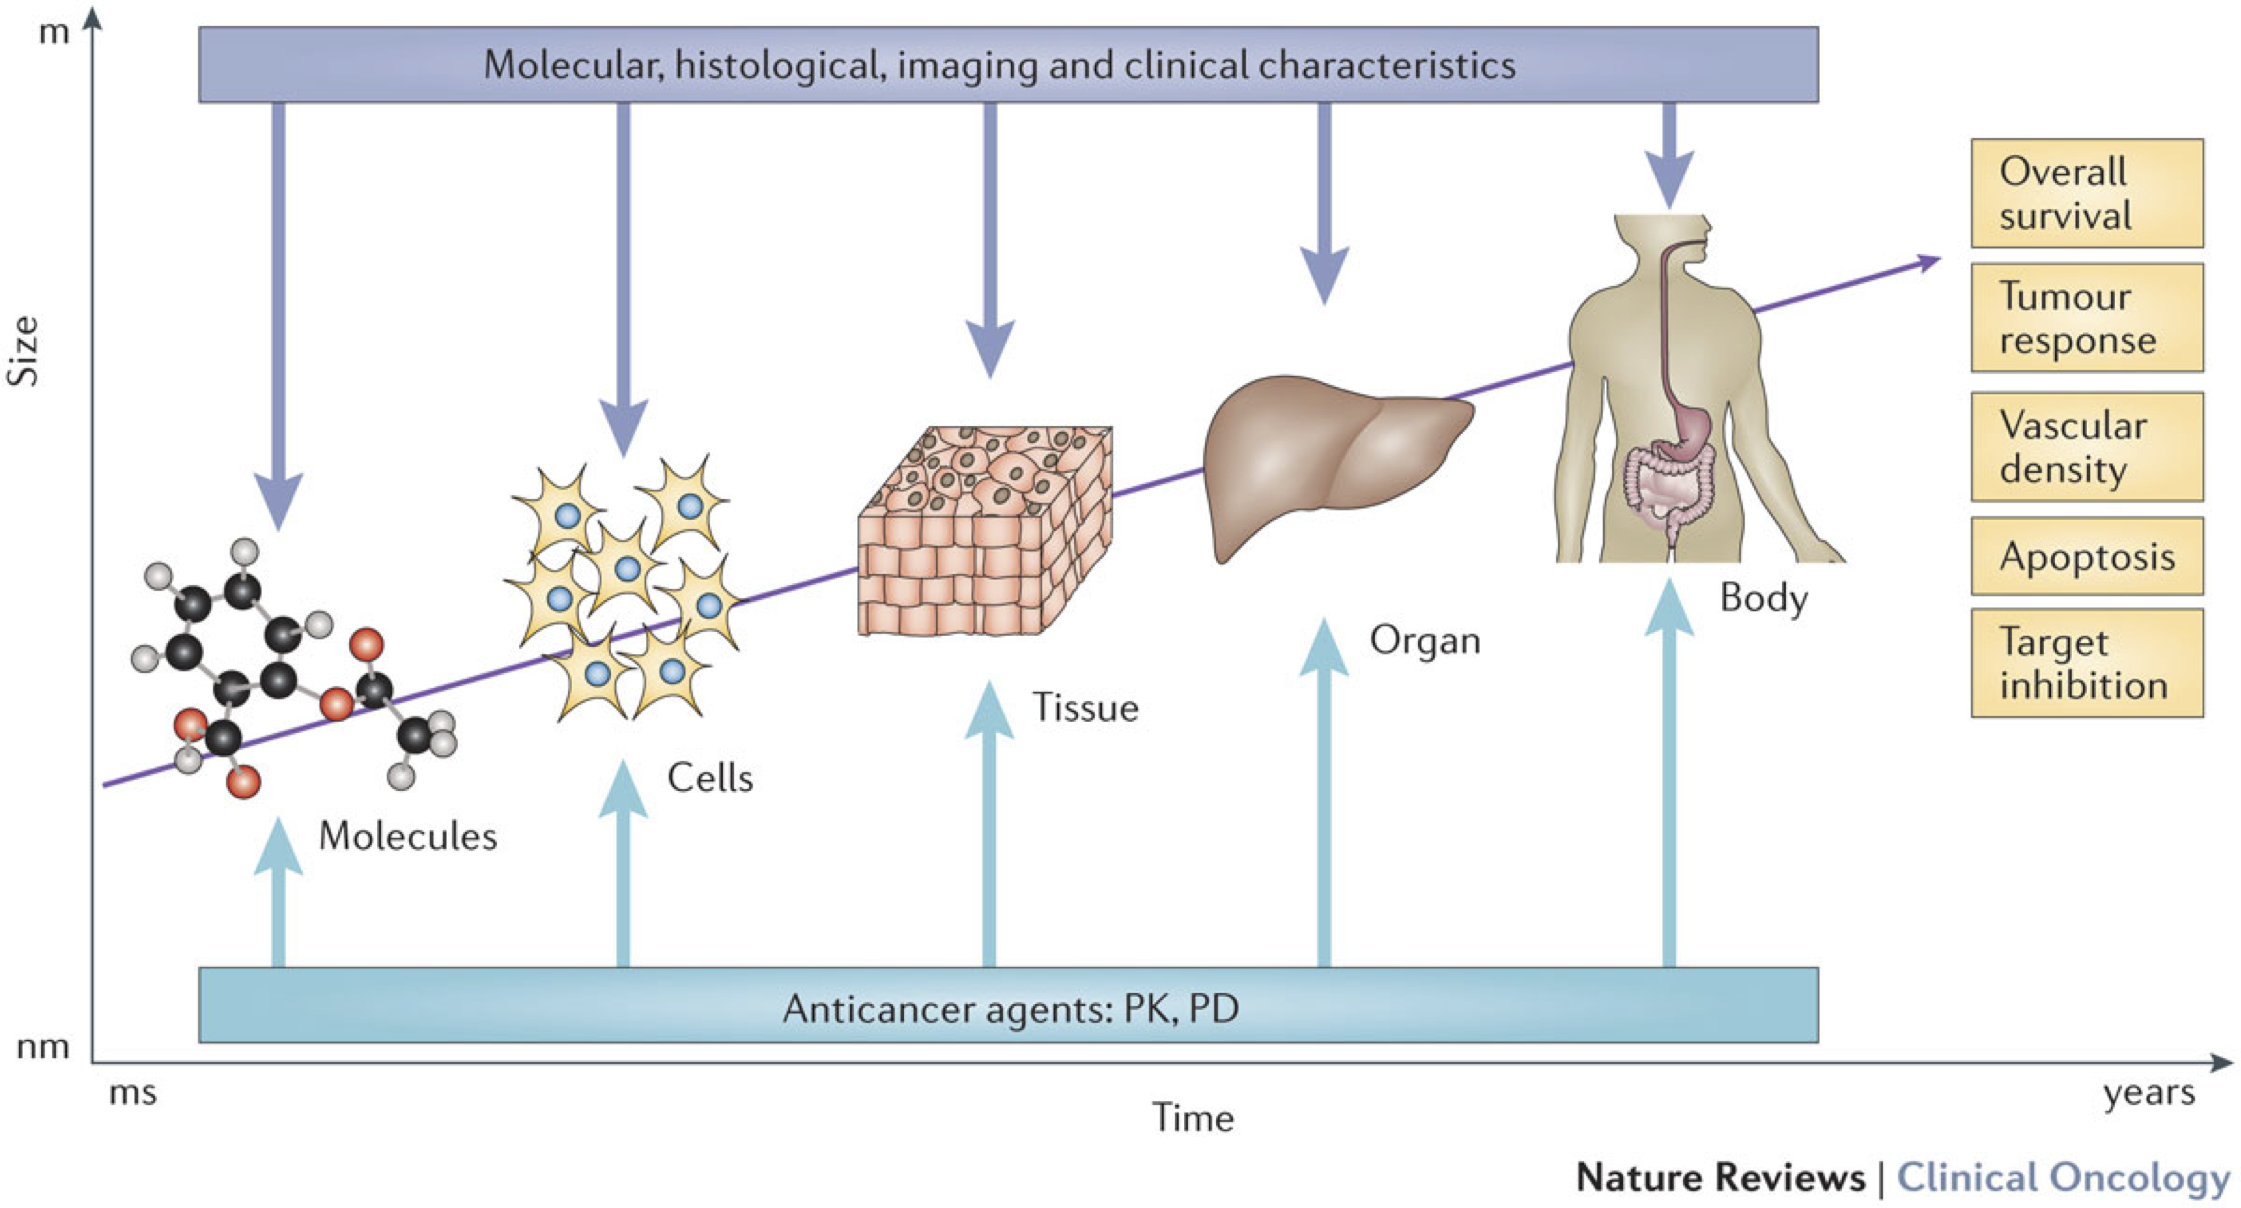
\includegraphics[width=0.9\linewidth]{fig/multiscale} 

}

\caption[The different scales of cancer modeling]{\textbf{The different scales of cancer
modeling.} Cancer can be approached at different scales, from molecules
to organs, using different data (dark blue), but often with the direct
or indirect objective of contributing to the study of clinically
interpretable phenomena (yellow boxes), in particular by studying the
influence of anticancer agents (pale blue). Reprinted from
\citet{barbolosi2016computational}.}\label{fig:multiscale}
\end{figure}









Taking it down a step further, it is also possible to model cancer at
the \textbf{cellular level}, for example by looking at the clonal
evolution of cancer \citep{altrock2015mathematics}. The aim is then to
understand the impact of the processes of mutation, selection, expansion
and cohabitation of different populatons of cells, at specifc rates. The
accumulation of a mutation in a population of cells can thus be studied
\citep{bozic2010accumulation}. Modeling at the cellular level is well
suited to the study of interactions between cells, between cancer cells
and their environment or with the immune system. Similar to other kinds
of studies of population dynamics, formalisms based on differential
equations are quite common \citep{bellomo2008foundations}; but there are
many other methods such partial differential equations or agent-based
modeling \citep{letort2019physiboss}.

Finally, at an even smaller scale, it is possible to model the
\textbf{molecular networks} at work in cells \citep{le2015quantitative}.
The aim is then to simulate mathematically how the different genes and
molecules regulate each other, transmit information and, in the case of
cancer, end up being deregulated \citep{calzone2010mathematical}. These
models will be the subject of the thesis and will therefore be defined
more precisely and used to detail the concepts and tools of systems
biology in the following sections. It can already be noted that while
these models can integrate the most fundamental biological mechanisms of
living organisms, one of the most burning questions is whether it is
possible to link them to the larger scales that are clinically more
interesting (tissues, organs etc.). Can these models tell us something
about the molecular nature of cancer? About patient survival? Their
response to treatment? These questions apply to all of the above models,
whatever their scales (Figure \ref{fig:multiscale}), but are more
difficult to answer for models defined at molecular scale that are
further from the clinical data of interest. The aim of this thesis is to
provide potential answers to these questions. One of the ways of
approaching these issues has been to propose multi-scale models, which
are nevertheless very complex
\citep{anderson2008integrative, powathil2015systems}. We will focus here
on the use of models defined almost exclusively at the molecular scale,
which is assumed to be prominent, to study what can be inferred on the
larger scales.

\section{Cell circuitry and the need for cancer systems
biology}\label{cell-circuitry-and-the-need-for-cancer-systems-biology}

Most biological systems, and certainly cells, fall into the category of
\textbf{complex systems}. These are systems made up of many interacting
elements. While these systems can be found in many different scientific
fields, the cell as a complex system is characterized by the diversity
and multifunctionality of its constituent elements (genes, proteins,
small molecules, enzymes), which nevertheless contribute to organized
and a priori non-chaotic behaviour \citep{kitano2002computational}.
Thus, the role of a protein such as the p53 tumour suppressor can only
be understood by taking into account the interplay between its
relationships with transcription factors and biochemical modifications
of the molecule itself \citep{kitano2002computational}. In a cell, as in
any complex system, the multiplication of components and interactions
can make the response or behaviour of the system unexpected or
unpredictable. Non-linear responses, such as abrupt changes in the state
of a system, called critical transitions, can be observed in response to
a moderate change in the signal \citep{trefois2015critical}. Generally
speaking, it is possible to observe \textbf{emergent behaviours},
i.e.~behaviours of the system as a whole that were not trivially
deducible from the individual behaviours of its components. This has
been documented, through experiments and simulations, in the study of
cell signalling pathways and the resulting biological decisions
\citep{bhalla1999emergent, helikar2008emergent}. These considerations
have thus given rise to \textbf{system-level or holistic approaches that
aim to integrate data and knowledge into more comprehensive
representations, often called systems biology}.

What is true for the cell in general is just as true for cancer in
particular. Understanding the intertwining of signaling pathways is
necessary to study their contributions to different cancer hallmarks, as
shown in Figure \ref{fig:circuit}. The concepts described above can thus
be transposed to \textbf{cancer systems biology}
\citep{hornberg2006cancer, kreeger2010cancer, barillot2012computational}.
Indeed, it is often a question of understanding or predicting the impact
of perturbations on cellular networks. Understanding how a single
genetic mutation disrupts and reprograms networks, or even predicting
the responses triggered by a drug on a presumably promising molecular
target, makes little sense without integrated approaches. In addition,
cancers are characterized by the accumulation of numerous mutations and
alterations over time that must be considered concomitantly. These
points of view of biologists and modellers reinforce the observation
already made in the previous chapter of cancer as a network disease, as
a system disease (Figure \ref{fig:pathways}).

Finally, to conclude this general presentation, it is important to
understand that while small molecular network modeling is not recent,
the rise and multiplication of wide range systems biology approaches is
very much related to the production of biological data
\citep{de2002modeling}. The last few decades have seen the emergence of
high-throughput data that have made it possible to identify and link
hundreds of genes or proteins involved in cancer. Exploring the
interaction and back and forth between these models and the data they
use or predict is therefore of utmost importance. In addition, the now
** massive amount of data has also imposed mathematical or computational
approaches as a central element in the management of this profusion**
and more and more modeling approaches are focused on data integration or
inference \citep{frohlich2018efficient, bouhaddou2018mechanistic}. More
generally, Figure \ref{fig:pubmed} shows that while the number of
scientific articles devoted to cancer has increased drastically since
the 1950s (panel A), the proportion of these same articles mentioning
\emph{models}, \emph{networks} or \emph{computational} approaches has
also increased (panel B), illustrating a change in paradigms.

\begin{figure}

{\centering 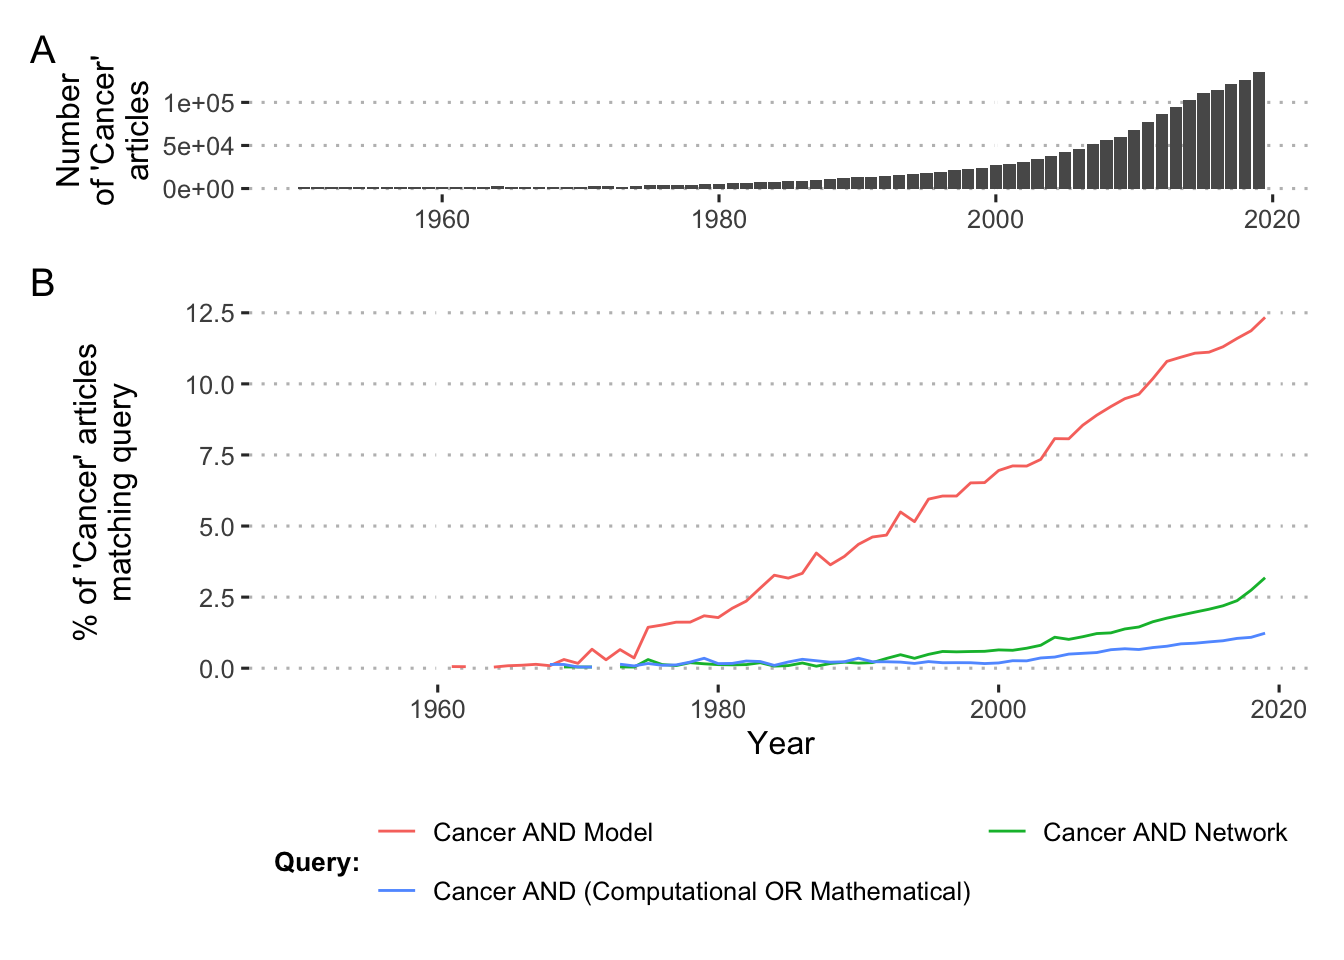
\includegraphics[width=0.9\linewidth]{03-Mechanistic_files/figure-latex/pubmed-1} 

}

\caption[PubMed trends in cancer studies.]{\textbf{PubMed trends in cancer studies.} (A)
PubMed articles with the word \emph{Cancer} in either title or abstract
from 1950 to 2019. (B) Proportion of the \emph{Cancer} articles with
additional keywords expressed as PubMed logical queries.}\label{fig:pubmed}
\end{figure}






\section{Mechanistic models of molecular
signaling}\label{mechanistic-models-of-molecular-signaling}

Once the context has been defined, both biologically and
methodologically, it is possible to begin the exploration of the models
that will constitute the core of this thesis: the \textbf{mechanistic
models of molecular networks} and signaling pathways. Before describing
and illustrating some of the existing mathematical formalisms, it is
possible to describe the common fundamental elements of this family of
approaches.

\subsection{Networks and data}\label{networks-and-data}

The first step is to identify the relevant biological entities from a
question or system of interest (e.g.~tumor suppressor genes, signaling
cascades of proteins) and then to model their interactions, the
regulatory relationships that link them. At this stage the model can
generally be represented by a network but this word can cover different
realities \citep{le2015quantitative}. The simplest network just
represents undirected interactions between entities, which therefore
only establishes relationships and not causal mechanisms. But modeling
requires more precise definitions, in particular concerning the
direction of the interaction (is it A that acts on B or the opposite)
and its nature (type of chemical reaction, activation/inhibition etc.).
This is usually summarized as \textbf{activity flows (or influence
diagrams) with activation and inhibition arrows} as in Figure
\ref{fig:circuit} or Figure \ref{fig:toyraf}A. These arrows emphasize
the transormation of static networks into dynamic objects that can be
manipulated and interpreted mechanistically. This work can be taken
further by writing bipartite graphs, known as process descriptions,
which explicitly show the different states of each variable (first type
of nodes), depending on their phosphorylation sate for instance, and the
reactions that link them (second type of nodes) as in Figure
\ref{fig:toyraf}B. A more precise description of these different
representations and their meanings can be found in
\citet{le2015quantitative}. \textbf{Once the network structure of the
model has been defined, it is possible write the corresponding
mathematical formalism} and potentially to refine certain parameters.
Finally, the model is often confronted with new data to check its
consistency with the biological behaviour studied or possibly make new
predictions.

However, all these steps are not linear and sequential, but rather
iterative and cyclical. This \textbf{modeling cycle}, with back and
forth to the data, is not specific to molecular network models, but it
is possible to specify it in this case (Figure \ref{fig:cycle}). The
names of the key players involved in the question of interest are thus
first extracted from adapted data or from the literature. A first
mathematical translation of the relationships between the entities is
then proposed before verifying the compatibility of this model with the
observations, whether qualitative or quantitative. If the compatibility
is not good, we come back to the definition or the parameterization of
the model. If compatibility is correct, the model can be used to make
new predictions or study phenomena that go beyond the initial data set.
Ideally, these predictions will be tested afterwards. This cyclic
approach with two successive checks is analogous to the use of
validation and test data in the evaluation of most learning algorithms.
This analogy can sometimes be masked by the qualitative nature of the
predictions or by the lack of explicit fitting of the parameters.

\begin{figure}

{\centering 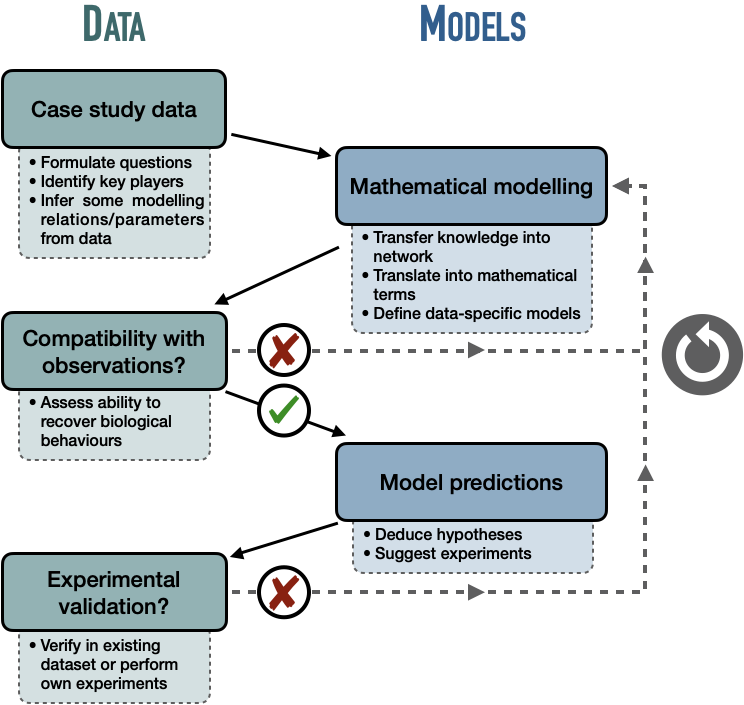
\includegraphics[width=0.7\linewidth]{fig/cycle} 

}

\caption[Modeling a biological network: an iterative and cyclical process]{\textbf{Modeling a biological network: an iterative
and cyclical process.} Reprinted from \citep{beal2020modelisation}. A
different and simpler version of this cycle is described in
\citep{le2015quantitative}.}\label{fig:cycle}
\end{figure}






\subsection{Different formalisms for different
applications}\label{different-formalisms-for-different-applications}

Beyond these similarities in the construction and representation of
models, the precise mathematical formalism that underlies them varies
according to the type of question and the data \citep{de2002modeling}.
For the sake of simplicity, and without exhaustiveness, we propose to
divide into quantitative and qualitative formalisms which will be
essentially illustrated respectively by \textbf{ordinary differential
equation (ODE)} models and \textbf{logical (or Boolean) models} for
which a graphical and schematic comparison is proposed in Figure
\ref{fig:toyraf}.

\begin{figure}

{\centering 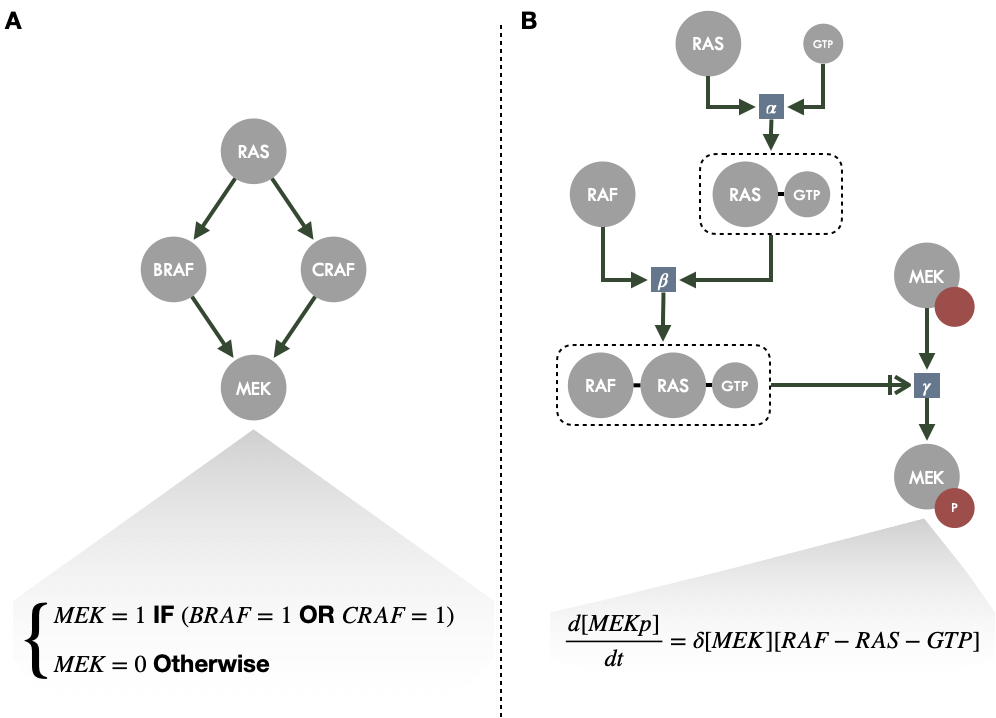
\includegraphics[width=0.9\linewidth]{fig/toyraf} 

}

\caption[Schematic example of logical and ODE modeling around MAPK signaling]{\textbf{Schematic example of logical and ODE
modeling around MAPK signaling.} (A) Activity flow diagram of a small
part of MAPK signaling, each node representing a gene or protein, with
an example of logical rule for MEK node for the corresponding logical
model. (B) Process description of the same diagram with BRAF and CRAF
merged in RAF for the sake of simplicity; each square representing a
reaction and the correspondong rate; an example differential equation is
provided for the phosphorylated (active) form of MEK.}\label{fig:toyraf}
\end{figure}










One of the most frequent approaches is the use of \textbf{chemical
kinetics} equations to construct ODE systems which are a fairly natural
translation of the process descritption networks described in the
previous section \citep{polynikis2009comparing}. Each biological
interaction is treated as a reaction governed by the law of mass action
and, under certain hypotheses, as a differential equation (Figure
\ref{fig:toyraf}B); the set of reactions in the system then generates a
set of differential equations with coupled variables, in an analogous
way to the Lotka Volterra system presented in section
\ref{lotkasection}. Thus the variables generally represent quantities of
molecular species, for example concentrations of RNA or proteins, and
the stoichiometric coefficients and reaction rates are used to define
the system parameters. Approximations are sometimes made to simplify the
equations, for example by assuming that they can be written as
Michaelis-Menten's enzymatic reactions, which have a simple and well
known behaviour. However, the theoretical accuracy of quantitative
models has a cost since \textbf{each differential equation requires
parameters}, such as reaction constants or initial conditions, to which
the system is very sensitive \citep{le2015quantitative}. The biochemical
interpretation of the parameters sometimes allow to find their value in
the literature, if the reactions are well characterized, even if
possible variations in a given biological or physical context are often
unknown. Since knowledge of the values of these parameters is often
limited or even non-existent, it may require a very large volume of data
(including time series) to fit the many missing parameters which can be
difficult if the number of parameters is large
\citep{villaverde2014reverse}. However, recent work has demonstrated the
feasibility and scalability of this type of inference with sufficiently
rich data \citep{frohlich2018efficient}.

At the same time, more qualitative approaches to modeling biological
networks have been proposed with discrete variables linked together by
rules expressed as logical statements \citep{abou2016logical}. These
models are both more abstract since variables do not have a direct
biological interpretation (e.g.~concentration of a species) but are more
versatile since they can unify different biological realities under the
same formalism (e.g.~activation of a gene or phosphorlation of a
protein). The discrete nature of the variables can then be seen as an
asymptotic case of the sigmoidal (e.g.~Hill function) relationships
often found in biology \citep{le2015quantitative}. The step function
thus obtained can keep a natural interpretation in the context of
biological phenomena: genes activated or not, protein present or absent
etc. Similarly, interactions between species are not quantified but are
based on a qualitative statements (e.g.~A will be active if B and C are
active), drastically reducing the number of parameters (Figure
\ref{fig:toyraf}A). If the theoretical interest of this formalism to
study biological mechanisms was proposed quite early
\citep{kauffman1969homeostasis, thomas1973boolean}, many concrete
applications have also been developed over the years, particularly in
cancer research \citep{saez2011comparing, remy2015modeling}. This
\textbf{logical formalism will constitute the core of the work presented
in Part II}, where it will therefore be discussed in greater detail.

\begin{table}

\caption{\label{tab:odelogic}\textbf{Features of quantitative and qualitative
modeling applied to biological molecular networks} (adapted from
\citet{le2015quantitative})}
\centering
\begin{tabular}[t]{>{\bfseries\raggedright\arraybackslash}p{6em}||>{\raggedright\arraybackslash}p{12em}|>{\raggedright\arraybackslash}p{12em}}
\hline
\rowcolor[HTML]{808080}  \multicolumn{1}{c}{\textcolor{white}{\textbf{ }}} & \multicolumn{1}{c}{\textcolor{white}{\textbf{Quantitative modeling}}} & \multicolumn{1}{c}{\textcolor{white}{\textbf{Qualitative modeling}}}\\
\hline
Example formalism & Ordinary differential equation (ODE) models & Logical models\\
\hline
Type of variables & Direct translation of biological quantities, usually continuous & Abstract representation of activity levels, usually discrete\\
\hline
Objective & Quantitatively accurate and temporal simulation of an experimental phenomenon & Coarse-grained simulation of qualitative phenotypes\\
\hline
Advantages & Direct confrontation with experimental data; precise; linear representation of time & Faster design; easy translation of literature-based assertions; simulation of perturbations\\
\hline
Drawbacks & Difficulty determining or fitting parameters & More difficult to link to data; lower precision\\
\hline
\end{tabular}
\end{table}





These two formalisms, which are among the most frequent for modelling
biological networks, share many similarities, in particular the
propensity to be built according to bottom-up strategies based on
knowledge of the elementary parts of the model, i.e.~biological entities
and reactions. However, they differ in their implementation and
objectives, \textbf{one aiming at the most accurate representation
possible, the other seeking to capture the essence of the system's
dynamics in a parsimonious way} (Table \ref{tab:odelogic}). The
opposition is not irrevocable, as illustrated by the numerous hybrid
formalisms that lie within the spectrum delimited by these two extremes
such as fuzzy logic or discrete-time differential equations
\citep{le2015quantitative, calzone2018logical}. To conclude, a
comparison between the two approaches applied to the same problem is
proposed by \citet{calzone2018logical}, studying the
epithelio-mesenchymal transition (EMT, a biological process involved in
cancer), to illustrate in concrete terms their complementarity.

\subsection{Some examples of complex
features}\label{some-examples-of-complex-features}

With the help of these models, both qualitative and quantitative, many
complex behaviours have been identified. Benefiting from the knowledge
accumulated in the study of dynamic systems, a whole zoo of patterns
with complex and non-intuitive behaviours such as non-linearities have
been highlighted \citep{tyson2003sniffers}. The MAPK pathway, coarsely
described in Figure \ref{fig:toyraf}, and often simplified as a rather
unidirectional cascade, shows switch or bistability behaviors generated
by the complexity of its multiple phosphorylation sites
\citep{markevich2004signaling}. These models have also been put at the
service of understanding cancer and the erroneous decision-making by
cells resulting from impaired signaling pathways. Thus,
\citet{tyson2011dynamic} summarize superbly well the complexity that can
be hidden in the dynamics of smallest molecular networks as soon as they
contain more than two entites and crossed regulations or feedback loops.
Logical models have also made it possible to better dissect some complex
phenomena at play in the cell such as emergent behaviours
\citep{helikar2008emergent} or mechanisms behind mutation patterns in
cancer \citep{remy2015modeling}.

\section{From mechanistic models to clinical
impact?}\label{from-mechanistic-models-to-clinical-impact}

Mechanistic models have therefore undeniably led to a better
understanding of the complex molecular machinery of signalling pathways.
But beyond the interest that this understanding represents, do these
models also have a clinical utility? In other words, \textbf{are they of
clinical or only scientific value?}

\subsection{A new class of biomarkers}\label{a-new-class-of-biomarkers}

Throughout this thesis, the clinical value of mechanical models will
often be analyzed by analogy to that of biomarkers. Throughout this
thesis, the clinical value of mechanical models will often be analyzed
by analogy to that of biomarkers. Biomarkers are usually defined as
measurable indicators of patient status or disease progression, such as
prostate-specific antigen (PSA) for prostate cancer screening or BRCA1
mutation for breast cancer risk \citep{henry2012cancer}. Biomarkers also
encompass multivariate signatures that identify more complex patterns
with clinical significance. Taking the logic even further, it was
therefore proposed that mechanistic models, which also reveal complex
molecular behaviours, could be considered as biomarkers, capturing
perhaps even dynamic information \citep{fey2015signaling}.

Like oncology biomarkers, the models will be divided into two categories
according to their clinical objectives: \textbf{prognostic models and
predictive models} \citep{oldenhuis2008prognostic}. Prognostic
biomarkers and models are those that provide information on the
evolution of cancer independently of treatment. They are therefore
generally confronted with survival or relapse data. The protein Ki-67
for example, encoded by the MKI67 gene, is known to be indicative of the
level of proliferation and high levels of expression are thus associated
with a poorer prognosis in many cancers \citep{sawyers2008cancer}.
Predictive biomarkers and models, on the other hand, give an indication
of the effect of a therapeutic strategy. The simplest example, but not
the only one, concerns biomarkers that are themselves the target of
treatment: treatments based on monoclonal antibodies directed against
HER2 receptors in breast cancer are only effective if the HER2 receptor
has been detected in the patient \citep{sawyers2008cancer}. Without
attempting to be exhaustive, some logical and ODE models, with either
prognostic or predictive claims, will be described.

\subsection{Prognostic models}\label{prognostic-models}

One of the first mechanical models of cell signalling to have been
explicitly presented as a prognostic biomarker is the one proposed by
\citet{fey2015signaling} and describing c-Jun N-terminal kinase (JNK)
pathway in neuroblastoma cells. A summary of the study is provided in
Figure \ref{fig:fey}). The model is an ODE translation of the process
description network of Figure \ref{fig:fey})A, further determined and
calibrated with molecular biology experimental data obtained using
neuroblastoma cell lines. We thus observe the non-linear switch-like
dynamics of JNK activation as a function of cellular stress (Figure
\ref{fig:fey})B). The precise characteristics of this sgmoidal response
can, however, vary from one individual to another as captured by the
network output descriptors \(A\), \(K_{50}\) and \(H\). Fey et al.
proposed to perform neuroblastoma patient--specific simulations of the
model, using patient gene expressions for ZAK, MKK4, MKK7, JNK and AKT
genes to specify the initial conditions of the ODE system. Since JNK
activation induces cell death through apoptosis, the patient-specific
\(A\), \(K_{50}\) and \(H\) derived from patient-specifc models are then
analyzed as prognostic biomarkers (Figure \ref{fig:fey})C). Readers are
invited to refer to the original article for details on model
calibration or binarization of network descriptors
\citep{fey2015signaling}. The authors also showed that in the absence of
positive feedback from \(JNK^{**}\) to \(^PMKK7\), an important
component of non-linearity, the prognostic value is drastically
decreased. All in all, this pipeline from ODE model to survival curves,
thus provides a \textbf{paradigmatic example of the clinical
interpretation of mechanistic models of molecular networks} that will be
reused in later chapters for illustration purposes. Other ODE models
following a similar rationale have been proposed by the same group for
colorectal cancer \citep{hector2012clinical, salvucci2017stepwise} or
glioblastoma {[}\citet{murphy2013activation}; salvucci2019system{]}.
Machine learning approaches have also been proposed to ease the clinical
implementation of this kind of prognostic models by dealing with the
potential lack of patient data needed to personalize them
\citep{salvucci2019machine}.

\begin{figure}

{\centering 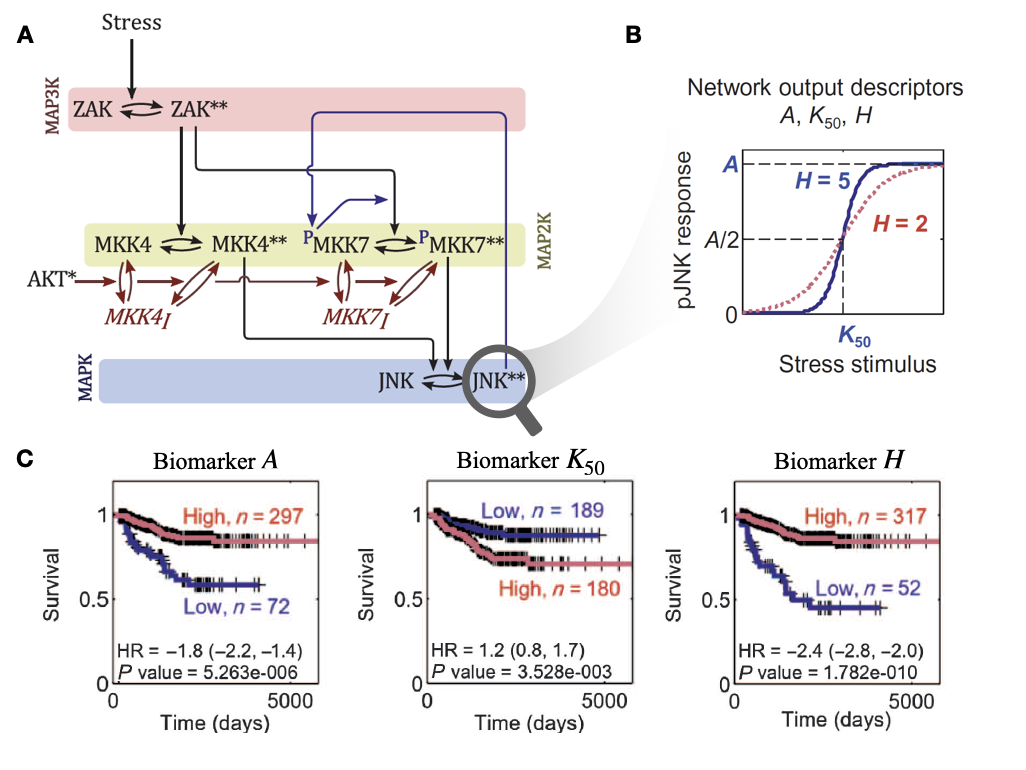
\includegraphics[width=0.9\linewidth]{fig/fey} 

}

\caption[Schematic example of logical and ODE modeling around MAPK signaling]{\textbf{Mechanistic modeling of JNK pathway and
survival of neuroblastima patients, as described by
\citet{fey2015signaling}.} (A) Schematic representation, as a process
description, for the ODE model of JNK pathway. (B) Response curve
(phosphorylated JNK) as a function of the input stimulus (Stress) and
characterization of the corresponding sigmoidal function with maximal
amplitude \(A\), Hill exponent \(H\) and activation threshold
\(K_{50}\). (C) Survival curves for neuroblastoma patients based on
binarized \(A\), \(K_{50}\) and \(H\); binarization thresholds having
been defined based on optimization screening on calibration cohort.}\label{fig:fey}
\end{figure}












On the logical modeling side, there are also studies including
prognostic value validation. Thus, \citet{khan2017unraveling} proposed
two logical models of epitelio-mesenchymal transition (EMT) in bladder
and breast cancers. These models are inferred from prior mechanisms
knowledge and data analysis with particular attention to potential
feedback loops. Using these models, it is possible to study the
behaviour of them for all combinations of model inputs (growth factors
and receptor proteins) and derive subsequent signatures for good or bad
prognosis. These signatures are later validated with cohorts of
patients. In this case, the mechanistic model does not seek to capture a
dynamic behavior but to facilitate and \textbf{make understandable the
exploration of combinations of input signals that grow exponentially
with the number of inputs considered}. Other formalisms, called pathway
activity analysis and following the same activity flows principles
(Figure \ref{fig:toyraf}A), have been analysed in the light of their
prognostic value. Their greater flexibility enables the direct use of
networks of several hundred or thousands of genes, such as those present
in the KEGG database \citep{kanehisa2012kegg}. The benefit of
mechanistic modeling is then to organize high-dimensional data and to
facilitate the \emph{a posteriori} analysis of the results.

\subsection{Predictive models}\label{predictive-models}

But the explicit representation of biological entities in mechanistic
models makes them particularly \textbf{suitable for the study of
well-defined perturbations such as drug effects}. Indeed, by assuming
that the mechanism of action of a drug is at least partially known, it
is possible to integrate this mechanism into the model if it contains
the target of the drug (Figure \ref{fig:netdrug}). One can therefore
simulate the effect of one drug or even compare several. These
strategies have already been implemented in a qualitative way with
logical models used to explain resistance to certain treatments of
breast cancer \citep{zanudo2017network} or even highlight the synergy of
certain combinations of treatments in gastric cancer
\citep{flobak2015discovery}. The value of these models, however, is more
scientific than clinical in that they focus on a single cell line or a
restricted group of cell lines. The possibility to personalize the
predictions or recommendations for different molecular profiles of cell
lines or patients is therefore not obvious. Still within the context of
logical formalism, \citet{knijnenburg2016logic} proposed a broader
approach: if their model needs to be trained, it can nevertheless
provide an analytical framework for several hundred cell lines, while
remaining within the scope of the training data to ensure the validity
of predictions.

\begin{figure}

{\centering 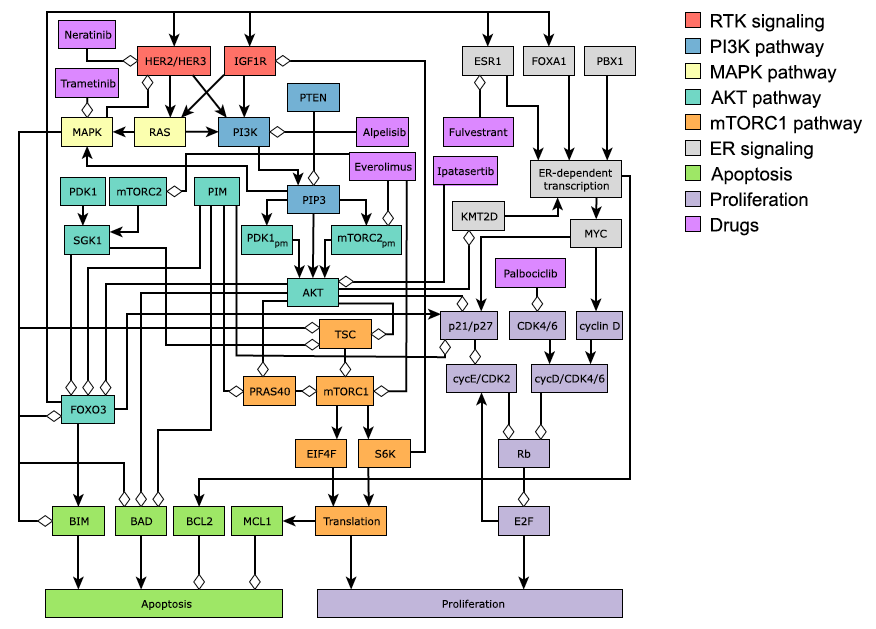
\includegraphics[width=0.9\linewidth]{fig/netdrug} 

}

\caption[Network model of oncogenic signal transduction in ER+ breast cancer, including some drugs and their targets]{\textbf{Network model of oncogenic signal
transduction in ER+ breast cancer, including some drugs and their
targets.} Reprinted from \citet{zanudo2017network}.}\label{fig:netdrug}
\end{figure}





Conceptually comparable strategies can be found on the side of
differential equations where large mechanical models of cell signalling
are also trained to predict the response to different treatments
\citep{bouhaddou2018mechanistic, frohlich2018efficient}. A calibrated
model can then predict the response to a combination of treatments not
tested in the training data, thereby proving the ability of mechanistic
models to extend their predictive value beyond the data
\citep{frohlich2018efficient}. As with prognostic models, mechanical
approaches other than logical formalisms and ODEs have been proposed and
validated \citep{jastrzebski2018integrative}. What can be learned from
these predictive models is that they require \textbf{significant
training data to be able to go beyond qualitative predictions and
dissect treatment response mechanisms of many cell lines
simultaneously}. For obvious practical and ethical reasons, the
validation of these models is for the moment limited to preclinical data
since they require data for many uncertain therapeutic interventions.

This first bridge between mechanistic models of cell signalling and
clinical applications concludes this introductory part. The next part
will be devoted to the definition of new methods to establish this
connection based on logical formalism, before the third part proposes a
more statistical evaluation of the prognostic and predictive values of
the models presented in the previous parts.

\chapter{Test part}\label{test}

This is a test

\section{Test}\label{test}

\bibliography{bib/thesis.bib}

\end{document}
